\documentclass[twoside]{book}

% Packages required by doxygen
\usepackage{fixltx2e}
\usepackage{calc}
\usepackage{doxygen}
\usepackage[export]{adjustbox} % also loads graphicx
\usepackage{graphicx}
\usepackage[utf8]{inputenc}
\usepackage{makeidx}
\usepackage{multicol}
\usepackage{multirow}
\PassOptionsToPackage{warn}{textcomp}
\usepackage{textcomp}
\usepackage[nointegrals]{wasysym}
\usepackage[table]{xcolor}

% Font selection
\usepackage[T1]{fontenc}
\usepackage[scaled=.90]{helvet}
\usepackage{courier}
\usepackage{amssymb}
\usepackage{sectsty}
\renewcommand{\familydefault}{\sfdefault}
\allsectionsfont{%
  \fontseries{bc}\selectfont%
  \color{darkgray}%
}
\renewcommand{\DoxyLabelFont}{%
  \fontseries{bc}\selectfont%
  \color{darkgray}%
}
\newcommand{\+}{\discretionary{\mbox{\scriptsize$\hookleftarrow$}}{}{}}

% Page & text layout
\usepackage{geometry}
\geometry{%
  a4paper,%
  top=2.5cm,%
  bottom=2.5cm,%
  left=2.5cm,%
  right=2.5cm%
}
\tolerance=750
\hfuzz=15pt
\hbadness=750
\setlength{\emergencystretch}{15pt}
\setlength{\parindent}{0cm}
\setlength{\parskip}{3ex plus 2ex minus 2ex}
\makeatletter
\renewcommand{\paragraph}{%
  \@startsection{paragraph}{4}{0ex}{-1.0ex}{1.0ex}{%
    \normalfont\normalsize\bfseries\SS@parafont%
  }%
}
\renewcommand{\subparagraph}{%
  \@startsection{subparagraph}{5}{0ex}{-1.0ex}{1.0ex}{%
    \normalfont\normalsize\bfseries\SS@subparafont%
  }%
}
\makeatother

% Headers & footers
\usepackage{fancyhdr}
\pagestyle{fancyplain}
\fancyhead[LE]{\fancyplain{}{\bfseries\thepage}}
\fancyhead[CE]{\fancyplain{}{}}
\fancyhead[RE]{\fancyplain{}{\bfseries\leftmark}}
\fancyhead[LO]{\fancyplain{}{\bfseries\rightmark}}
\fancyhead[CO]{\fancyplain{}{}}
\fancyhead[RO]{\fancyplain{}{\bfseries\thepage}}
\fancyfoot[LE]{\fancyplain{}{}}
\fancyfoot[CE]{\fancyplain{}{}}
\fancyfoot[RE]{\fancyplain{}{\bfseries\scriptsize Generated by Doxygen }}
\fancyfoot[LO]{\fancyplain{}{\bfseries\scriptsize Generated by Doxygen }}
\fancyfoot[CO]{\fancyplain{}{}}
\fancyfoot[RO]{\fancyplain{}{}}
\renewcommand{\footrulewidth}{0.4pt}
\renewcommand{\chaptermark}[1]{%
  \markboth{#1}{}%
}
\renewcommand{\sectionmark}[1]{%
  \markright{\thesection\ #1}%
}

% Indices & bibliography
\usepackage{natbib}
\usepackage[titles]{tocloft}
\setcounter{tocdepth}{3}
\setcounter{secnumdepth}{5}
\makeindex

% Hyperlinks (required, but should be loaded last)
\usepackage{ifpdf}
\ifpdf
  \usepackage[pdftex,pagebackref=true]{hyperref}
\else
  \usepackage[ps2pdf,pagebackref=true]{hyperref}
\fi
\hypersetup{%
  colorlinks=true,%
  linkcolor=blue,%
  citecolor=blue,%
  unicode%
}

% Custom commands
\newcommand{\clearemptydoublepage}{%
  \newpage{\pagestyle{empty}\cleardoublepage}%
}

\usepackage{caption}
\captionsetup{labelsep=space,justification=centering,font={bf},singlelinecheck=off,skip=4pt,position=top}

%===== C O N T E N T S =====

\begin{document}

% Titlepage & ToC
\hypersetup{pageanchor=false,
             bookmarksnumbered=true,
             pdfencoding=unicode
            }
\pagenumbering{roman}
\begin{titlepage}
\vspace*{7cm}
\begin{center}%
{\Large My Project }\\
\vspace*{1cm}
{\large Generated by Doxygen 1.8.11}\\
\end{center}
\end{titlepage}
\clearemptydoublepage
\tableofcontents
\clearemptydoublepage
\pagenumbering{arabic}
\hypersetup{pageanchor=true}

%--- Begin generated contents ---
\chapter{Class Index}
\section{Class List}
Here are the classes, structs, unions and interfaces with brief descriptions\+:\begin{DoxyCompactList}
\item\contentsline{section}{\hyperlink{structnode}{node} }{\pageref{structnode}}{}
\item\contentsline{section}{\hyperlink{structnode1}{node1} }{\pageref{structnode1}}{}
\item\contentsline{section}{\hyperlink{structnode__info}{node\+\_\+info} }{\pageref{structnode__info}}{}
\end{DoxyCompactList}

\chapter{File Index}
\section{File List}
Here is a list of all files with brief descriptions\+:\begin{DoxyCompactList}
\item\contentsline{section}{\hyperlink{Lab1_8c}{Lab1.\+c} }{\pageref{Lab1_8c}}{}
\end{DoxyCompactList}

\chapter{Class Documentation}
\hypertarget{classdice}{}\section{dice Class Reference}
\label{classdice}\index{dice@{dice}}
\subsection*{Public Member Functions}
\begin{DoxyCompactItemize}
\item 
\hyperlink{classdice_a928f9a4f4ba4ba2e6615aadc8d5a0de2}{dice} ()
\item 
int \hyperlink{classdice_a967f61248ffb11035c4b2f30b5c32bbb}{rolldice} (void)
\item 
\hyperlink{classdice_ab6557d0affda2992c8fc5578169a065b}{operator int} ()
\end{DoxyCompactItemize}
\subsection*{Private Attributes}
\begin{DoxyCompactItemize}
\item 
int \hyperlink{classdice_a7815c195f434449c65d2b242fbc54942}{dice1}
\end{DoxyCompactItemize}


\subsection{Constructor \& Destructor Documentation}
\index{dice@{dice}!dice@{dice}}
\index{dice@{dice}!dice@{dice}}
\subsubsection[{\texorpdfstring{dice()}{dice()}}]{\setlength{\rightskip}{0pt plus 5cm}void dice\+::dice (
\begin{DoxyParamCaption}
{}
\end{DoxyParamCaption}
)}\hypertarget{classdice_a928f9a4f4ba4ba2e6615aadc8d5a0de2}{}\label{classdice_a928f9a4f4ba4ba2e6615aadc8d5a0de2}

\begin{DoxyCode}
31 \{
32    \hyperlink{classdice_a7815c195f434449c65d2b242fbc54942}{dice1}=0;
33 \}
\end{DoxyCode}


\subsection{Member Function Documentation}
\index{dice@{dice}!operator int@{operator int}}
\index{operator int@{operator int}!dice@{dice}}
\subsubsection[{\texorpdfstring{operator int()}{operator int()}}]{\setlength{\rightskip}{0pt plus 5cm}dice\+::operator int (
\begin{DoxyParamCaption}
{}
\end{DoxyParamCaption}
)\hspace{0.3cm}{\ttfamily [inline]}}\hypertarget{classdice_ab6557d0affda2992c8fc5578169a065b}{}\label{classdice_ab6557d0affda2992c8fc5578169a065b}

\begin{DoxyCode}
26     \{
27        \textcolor{keywordflow}{return} \hyperlink{classdice_a7815c195f434449c65d2b242fbc54942}{dice1}/1;
28     \}
\end{DoxyCode}
\index{dice@{dice}!rolldice@{rolldice}}
\index{rolldice@{rolldice}!dice@{dice}}
\subsubsection[{\texorpdfstring{rolldice(void)}{rolldice(void)}}]{\setlength{\rightskip}{0pt plus 5cm}int dice\+::rolldice (
\begin{DoxyParamCaption}
\item[{void}]{}
\end{DoxyParamCaption}
)}\hypertarget{classdice_a967f61248ffb11035c4b2f30b5c32bbb}{}\label{classdice_a967f61248ffb11035c4b2f30b5c32bbb}

\begin{DoxyCode}
35 \{
36    randomize();
37    \hyperlink{classdice_a7815c195f434449c65d2b242fbc54942}{dice1}=rand()%6+1;
38    \textcolor{keywordflow}{return} \hyperlink{classdice_a7815c195f434449c65d2b242fbc54942}{dice1};
39 \}
\end{DoxyCode}


\subsection{Member Data Documentation}
\index{dice@{dice}!dice1@{dice1}}
\index{dice1@{dice1}!dice@{dice}}
\subsubsection[{\texorpdfstring{dice1}{dice1}}]{\setlength{\rightskip}{0pt plus 5cm}int dice\+::dice1\hspace{0.3cm}{\ttfamily [private]}}\hypertarget{classdice_a7815c195f434449c65d2b242fbc54942}{}\label{classdice_a7815c195f434449c65d2b242fbc54942}


The documentation for this class was generated from the following file\+:\begin{DoxyCompactItemize}
\item 
\hyperlink{SnakeAndLadder_8cpp}{Snake\+And\+Ladder.\+cpp}\end{DoxyCompactItemize}

\hypertarget{classplayer1}{}\section{player1 Class Reference}
\label{classplayer1}\index{player1@{player1}}
\subsection*{Public Member Functions}
\begin{DoxyCompactItemize}
\item 
\hyperlink{classplayer1_a6ccb31292781eb919f267a7f074aace0}{player1} ()
\item 
\hyperlink{classplayer1_a3ab242a781a3cdf6464805b7d343c743}{returna} ()
\item 
\hyperlink{classplayer1_adf9c92711824650060eab93ead7cdd36}{reseta} (int)
\item 
\hyperlink{classplayer1_ab39235bad6825ca38e4373924e492c85}{minusa} (int)
\item 
\hyperlink{classplayer1_ab9ea76c77f7ac22be75775b09c54d775}{operator int} ()
\end{DoxyCompactItemize}
\subsection*{Private Attributes}
\begin{DoxyCompactItemize}
\item 
int \hyperlink{classplayer1_a24d2b31ff59fa395160362ceb6f20099}{a}
\end{DoxyCompactItemize}


\subsection{Constructor \& Destructor Documentation}
\index{player1@{player1}!player1@{player1}}
\index{player1@{player1}!player1@{player1}}
\subsubsection[{\texorpdfstring{player1()}{player1()}}]{\setlength{\rightskip}{0pt plus 5cm}void player1\+::player1 (
\begin{DoxyParamCaption}
{}
\end{DoxyParamCaption}
)}\hypertarget{classplayer1_a6ccb31292781eb919f267a7f074aace0}{}\label{classplayer1_a6ccb31292781eb919f267a7f074aace0}

\begin{DoxyCode}
56 \{
57    \hyperlink{classplayer1_a24d2b31ff59fa395160362ceb6f20099}{a}=0;
58 \}
\end{DoxyCode}


\subsection{Member Function Documentation}
\index{player1@{player1}!minusa@{minusa}}
\index{minusa@{minusa}!player1@{player1}}
\subsubsection[{\texorpdfstring{minusa(int)}{minusa(int)}}]{\setlength{\rightskip}{0pt plus 5cm}int player1\+::minusa (
\begin{DoxyParamCaption}
\item[{int}]{ma}
\end{DoxyParamCaption}
)}\hypertarget{classplayer1_ab39235bad6825ca38e4373924e492c85}{}\label{classplayer1_ab39235bad6825ca38e4373924e492c85}

\begin{DoxyCode}
68 \{
69    \hyperlink{classplayer1_a24d2b31ff59fa395160362ceb6f20099}{a}-=ma;
70 \}
\end{DoxyCode}
\index{player1@{player1}!operator int@{operator int}}
\index{operator int@{operator int}!player1@{player1}}
\subsubsection[{\texorpdfstring{operator int()}{operator int()}}]{\setlength{\rightskip}{0pt plus 5cm}player1\+::operator int (
\begin{DoxyParamCaption}
{}
\end{DoxyParamCaption}
)\hspace{0.3cm}{\ttfamily [inline]}}\hypertarget{classplayer1_ab9ea76c77f7ac22be75775b09c54d775}{}\label{classplayer1_ab9ea76c77f7ac22be75775b09c54d775}

\begin{DoxyCode}
50     \{
51        \textcolor{keywordflow}{return} \hyperlink{classplayer1_a24d2b31ff59fa395160362ceb6f20099}{a}/1;
52     \}
\end{DoxyCode}
\index{player1@{player1}!reseta@{reseta}}
\index{reseta@{reseta}!player1@{player1}}
\subsubsection[{\texorpdfstring{reseta(int)}{reseta(int)}}]{\setlength{\rightskip}{0pt plus 5cm}int player1\+::reseta (
\begin{DoxyParamCaption}
\item[{int}]{ra}
\end{DoxyParamCaption}
)}\hypertarget{classplayer1_adf9c92711824650060eab93ead7cdd36}{}\label{classplayer1_adf9c92711824650060eab93ead7cdd36}

\begin{DoxyCode}
64 \{
65    \hyperlink{classplayer1_a24d2b31ff59fa395160362ceb6f20099}{a}+=ra;
66 \}
\end{DoxyCode}
\index{player1@{player1}!returna@{returna}}
\index{returna@{returna}!player1@{player1}}
\subsubsection[{\texorpdfstring{returna()}{returna()}}]{\setlength{\rightskip}{0pt plus 5cm}int player1\+::returna (
\begin{DoxyParamCaption}
{}
\end{DoxyParamCaption}
)}\hypertarget{classplayer1_a3ab242a781a3cdf6464805b7d343c743}{}\label{classplayer1_a3ab242a781a3cdf6464805b7d343c743}

\begin{DoxyCode}
60 \{
61    \textcolor{keywordflow}{return} \hyperlink{classplayer1_a24d2b31ff59fa395160362ceb6f20099}{a};
62 \}
\end{DoxyCode}


\subsection{Member Data Documentation}
\index{player1@{player1}!a@{a}}
\index{a@{a}!player1@{player1}}
\subsubsection[{\texorpdfstring{a}{a}}]{\setlength{\rightskip}{0pt plus 5cm}int player1\+::a\hspace{0.3cm}{\ttfamily [private]}}\hypertarget{classplayer1_a24d2b31ff59fa395160362ceb6f20099}{}\label{classplayer1_a24d2b31ff59fa395160362ceb6f20099}


The documentation for this class was generated from the following file\+:\begin{DoxyCompactItemize}
\item 
\hyperlink{SnakeAndLadder_8cpp}{Snake\+And\+Ladder.\+cpp}\end{DoxyCompactItemize}

\hypertarget{classplayer2}{}\section{player2 Class Reference}
\label{classplayer2}\index{player2@{player2}}
\subsection*{Public Member Functions}
\begin{DoxyCompactItemize}
\item 
\hyperlink{classplayer2_a9d0138199a3847deb0dcb813e7739d33}{player2} ()
\item 
\hyperlink{classplayer2_a32e37b8a129a947c0c037e0135c51c12}{returnb} ()
\item 
\hyperlink{classplayer2_a5d00283bc4c21a964bbd4149192b1537}{minusb} (int)
\item 
\hyperlink{classplayer2_a36cad9ccc12f3df2a45e2cf07f2ff1c7}{resetb} (int)
\item 
\hyperlink{classplayer2_a946a8ac3edee0b62c1b20fe9e94dad2d}{operator int} ()
\end{DoxyCompactItemize}
\subsection*{Private Attributes}
\begin{DoxyCompactItemize}
\item 
int \hyperlink{classplayer2_aabd15cdb6375642fc706adf650758589}{b}
\end{DoxyCompactItemize}


\subsection{Constructor \& Destructor Documentation}
\index{player2@{player2}!player2@{player2}}
\index{player2@{player2}!player2@{player2}}
\subsubsection[{\texorpdfstring{player2()}{player2()}}]{\setlength{\rightskip}{0pt plus 5cm}void player2\+::player2 (
\begin{DoxyParamCaption}
{}
\end{DoxyParamCaption}
)}\hypertarget{classplayer2_a9d0138199a3847deb0dcb813e7739d33}{}\label{classplayer2_a9d0138199a3847deb0dcb813e7739d33}

\begin{DoxyCode}
87 \{
88    \hyperlink{classplayer2_aabd15cdb6375642fc706adf650758589}{b}=0;
89 \}
\end{DoxyCode}


\subsection{Member Function Documentation}
\index{player2@{player2}!minusb@{minusb}}
\index{minusb@{minusb}!player2@{player2}}
\subsubsection[{\texorpdfstring{minusb(int)}{minusb(int)}}]{\setlength{\rightskip}{0pt plus 5cm}int player2\+::minusb (
\begin{DoxyParamCaption}
\item[{int}]{mb}
\end{DoxyParamCaption}
)}\hypertarget{classplayer2_a5d00283bc4c21a964bbd4149192b1537}{}\label{classplayer2_a5d00283bc4c21a964bbd4149192b1537}

\begin{DoxyCode}
100 \{
101    \hyperlink{classplayer2_aabd15cdb6375642fc706adf650758589}{b}-=mb;
102 \}
\end{DoxyCode}
\index{player2@{player2}!operator int@{operator int}}
\index{operator int@{operator int}!player2@{player2}}
\subsubsection[{\texorpdfstring{operator int()}{operator int()}}]{\setlength{\rightskip}{0pt plus 5cm}player2\+::operator int (
\begin{DoxyParamCaption}
{}
\end{DoxyParamCaption}
)\hspace{0.3cm}{\ttfamily [inline]}}\hypertarget{classplayer2_a946a8ac3edee0b62c1b20fe9e94dad2d}{}\label{classplayer2_a946a8ac3edee0b62c1b20fe9e94dad2d}

\begin{DoxyCode}
81     \{
82        \textcolor{keywordflow}{return} \hyperlink{classplayer2_aabd15cdb6375642fc706adf650758589}{b}/1;
83     \}
\end{DoxyCode}
\index{player2@{player2}!resetb@{resetb}}
\index{resetb@{resetb}!player2@{player2}}
\subsubsection[{\texorpdfstring{resetb(int)}{resetb(int)}}]{\setlength{\rightskip}{0pt plus 5cm}int player2\+::resetb (
\begin{DoxyParamCaption}
\item[{int}]{rb}
\end{DoxyParamCaption}
)}\hypertarget{classplayer2_a36cad9ccc12f3df2a45e2cf07f2ff1c7}{}\label{classplayer2_a36cad9ccc12f3df2a45e2cf07f2ff1c7}

\begin{DoxyCode}
96 \{
97    \hyperlink{classplayer2_aabd15cdb6375642fc706adf650758589}{b}+=rb;
98 \}
\end{DoxyCode}
\index{player2@{player2}!returnb@{returnb}}
\index{returnb@{returnb}!player2@{player2}}
\subsubsection[{\texorpdfstring{returnb()}{returnb()}}]{\setlength{\rightskip}{0pt plus 5cm}int player2\+::returnb (
\begin{DoxyParamCaption}
{}
\end{DoxyParamCaption}
)}\hypertarget{classplayer2_a32e37b8a129a947c0c037e0135c51c12}{}\label{classplayer2_a32e37b8a129a947c0c037e0135c51c12}

\begin{DoxyCode}
91 \{
92    \textcolor{keywordflow}{return} \hyperlink{classplayer2_aabd15cdb6375642fc706adf650758589}{b};
93 \}
\end{DoxyCode}


\subsection{Member Data Documentation}
\index{player2@{player2}!b@{b}}
\index{b@{b}!player2@{player2}}
\subsubsection[{\texorpdfstring{b}{b}}]{\setlength{\rightskip}{0pt plus 5cm}int player2\+::b\hspace{0.3cm}{\ttfamily [private]}}\hypertarget{classplayer2_aabd15cdb6375642fc706adf650758589}{}\label{classplayer2_aabd15cdb6375642fc706adf650758589}


The documentation for this class was generated from the following file\+:\begin{DoxyCompactItemize}
\item 
\hyperlink{SnakeAndLadder_8cpp}{Snake\+And\+Ladder.\+cpp}\end{DoxyCompactItemize}

\chapter{File Documentation}
\hypertarget{SnakeAndLadder_8cpp}{}\section{Snake\+And\+Ladder.\+cpp File Reference}
\label{SnakeAndLadder_8cpp}\index{Snake\+And\+Ladder.\+cpp@{Snake\+And\+Ladder.\+cpp}}
{\ttfamily \#include $<$dos.\+h$>$}\\*
{\ttfamily \#include $<$conio.\+h$>$}\\*
{\ttfamily \#include $<$stdio.\+h$>$}\\*
{\ttfamily \#include $<$stdlib.\+h$>$}\\*
{\ttfamily \#include $<$process.\+h$>$}\\*
{\ttfamily \#include $<$graphics.\+h$>$}\\*
{\ttfamily \#include $<$iostream.\+h$>$}\\*
Include dependency graph for Snake\+And\+Ladder.\+cpp\+:
\nopagebreak
\begin{figure}[H]
\begin{center}
\leavevmode
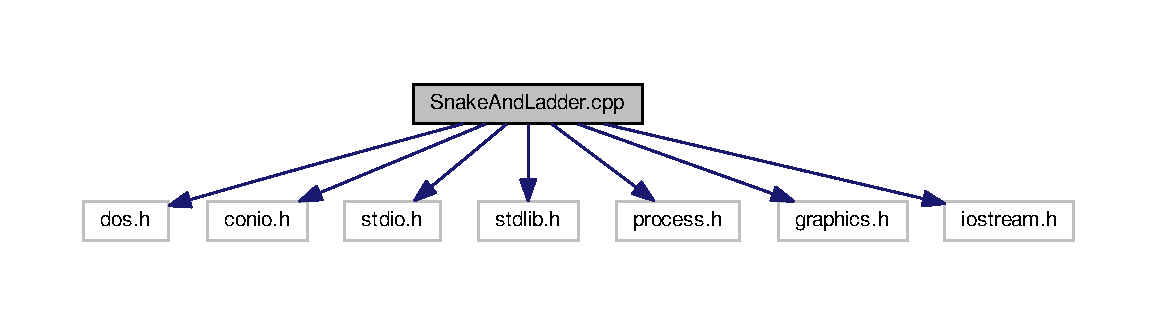
\includegraphics[width=350pt]{SnakeAndLadder_8cpp__incl}
\end{center}
\end{figure}
\subsection*{Classes}
\begin{DoxyCompactItemize}
\item 
class \hyperlink{classdice}{dice}
\item 
class \hyperlink{classplayer1}{player1}
\item 
class \hyperlink{classplayer2}{player2}
\end{DoxyCompactItemize}
\subsection*{Enumerations}
\begin{DoxyCompactItemize}
\item 
enum \hyperlink{SnakeAndLadder_8cpp_a38df57e4d2dd42645d8726b112528b77}{whoplays} \{ \hyperlink{SnakeAndLadder_8cpp_a38df57e4d2dd42645d8726b112528b77a22e7954f0f67bd13c875ccac1d77835d}{p1}, 
\hyperlink{SnakeAndLadder_8cpp_a38df57e4d2dd42645d8726b112528b77af023383ebe0126265f2dbaae87911cf9}{p2}
 \}
\end{DoxyCompactItemize}
\subsection*{Functions}
\begin{DoxyCompactItemize}
\item 
void \hyperlink{SnakeAndLadder_8cpp_ad7d433ae2456eac956adb9e68009763d}{graph} (int, int, int)
\item 
void \hyperlink{SnakeAndLadder_8cpp_a5602f1fbcedd7e2987edb6567dbc8a85}{sohaib} (void)
\item 
void \hyperlink{SnakeAndLadder_8cpp_a789894102928375db0a1992ef0faddf5}{ladder} (int, int, int, int)
\item 
void \hyperlink{SnakeAndLadder_8cpp_adc7531e628f13f194dbb35d5415df191}{cp1} (int, int)
\item 
void \hyperlink{SnakeAndLadder_8cpp_a83d10dadf87a53b425341460c6cb1b51}{cp2} (int, int)
\item 
void \hyperlink{SnakeAndLadder_8cpp_a49b806520ae2a5e43a36b121cb3a0e9c}{snake} (int, int, int, int)
\item 
\hyperlink{SnakeAndLadder_8cpp_a38df57e4d2dd42645d8726b112528b77}{whoplays} \hyperlink{SnakeAndLadder_8cpp_aba5a4315ee4edd33d8bf51cf2c5de467}{setplayer} (\hyperlink{SnakeAndLadder_8cpp_a38df57e4d2dd42645d8726b112528b77}{whoplays})
\item 
void \hyperlink{SnakeAndLadder_8cpp_acdef7a1fd863a6d3770c1268cb06add3}{main} ()
\end{DoxyCompactItemize}
\subsection*{Variables}
\begin{DoxyCompactItemize}
\item 
int \hyperlink{SnakeAndLadder_8cpp_a22d4ec3074b5dbbbc8a2225b7b23eead}{counter1} =0
\item 
int \hyperlink{SnakeAndLadder_8cpp_a4a83c833d1791f6e48fd7b0537ca23ec}{counter2} =0
\item 
int \hyperlink{SnakeAndLadder_8cpp_a949b553aaeb0f5233c17ed4feda5118c}{counter11} =0
\item 
int \hyperlink{SnakeAndLadder_8cpp_ab418db3d9c4875cda2de12f62792cdf1}{counter22} =0
\end{DoxyCompactItemize}


\subsection{Enumeration Type Documentation}
\index{Snake\+And\+Ladder.\+cpp@{Snake\+And\+Ladder.\+cpp}!whoplays@{whoplays}}
\index{whoplays@{whoplays}!Snake\+And\+Ladder.\+cpp@{Snake\+And\+Ladder.\+cpp}}
\subsubsection[{\texorpdfstring{whoplays}{whoplays}}]{\setlength{\rightskip}{0pt plus 5cm}enum {\bf whoplays}}\hypertarget{SnakeAndLadder_8cpp_a38df57e4d2dd42645d8726b112528b77}{}\label{SnakeAndLadder_8cpp_a38df57e4d2dd42645d8726b112528b77}
\begin{Desc}
\item[Enumerator]\par
\begin{description}
\index{p1@{p1}!Snake\+And\+Ladder.\+cpp@{Snake\+And\+Ladder.\+cpp}}\index{Snake\+And\+Ladder.\+cpp@{Snake\+And\+Ladder.\+cpp}!p1@{p1}}\item[{\em 
p1\hypertarget{SnakeAndLadder_8cpp_a38df57e4d2dd42645d8726b112528b77a22e7954f0f67bd13c875ccac1d77835d}{}\label{SnakeAndLadder_8cpp_a38df57e4d2dd42645d8726b112528b77a22e7954f0f67bd13c875ccac1d77835d}
}]\index{p2@{p2}!Snake\+And\+Ladder.\+cpp@{Snake\+And\+Ladder.\+cpp}}\index{Snake\+And\+Ladder.\+cpp@{Snake\+And\+Ladder.\+cpp}!p2@{p2}}\item[{\em 
p2\hypertarget{SnakeAndLadder_8cpp_a38df57e4d2dd42645d8726b112528b77af023383ebe0126265f2dbaae87911cf9}{}\label{SnakeAndLadder_8cpp_a38df57e4d2dd42645d8726b112528b77af023383ebe0126265f2dbaae87911cf9}
}]\end{description}
\end{Desc}

\begin{DoxyCode}
9 \{\hyperlink{SnakeAndLadder_8cpp_a38df57e4d2dd42645d8726b112528b77a22e7954f0f67bd13c875ccac1d77835d}{p1},\hyperlink{SnakeAndLadder_8cpp_a38df57e4d2dd42645d8726b112528b77af023383ebe0126265f2dbaae87911cf9}{p2}\};
\end{DoxyCode}


\subsection{Function Documentation}
\index{Snake\+And\+Ladder.\+cpp@{Snake\+And\+Ladder.\+cpp}!cp1@{cp1}}
\index{cp1@{cp1}!Snake\+And\+Ladder.\+cpp@{Snake\+And\+Ladder.\+cpp}}
\subsubsection[{\texorpdfstring{cp1(int, int)}{cp1(int, int)}}]{\setlength{\rightskip}{0pt plus 5cm}void cp1 (
\begin{DoxyParamCaption}
\item[{int}]{xx, }
\item[{int}]{yy}
\end{DoxyParamCaption}
)}\hypertarget{SnakeAndLadder_8cpp_adc7531e628f13f194dbb35d5415df191}{}\label{SnakeAndLadder_8cpp_adc7531e628f13f194dbb35d5415df191}

\begin{DoxyCode}
1463 \{
1464    setcolor(7);
1465    circle(xx,yy,10);
1466    setfillstyle(1,9);
1467    floodfill(xx,yy,7);
1468 \}
\end{DoxyCode}
\index{Snake\+And\+Ladder.\+cpp@{Snake\+And\+Ladder.\+cpp}!cp2@{cp2}}
\index{cp2@{cp2}!Snake\+And\+Ladder.\+cpp@{Snake\+And\+Ladder.\+cpp}}
\subsubsection[{\texorpdfstring{cp2(int, int)}{cp2(int, int)}}]{\setlength{\rightskip}{0pt plus 5cm}void cp2 (
\begin{DoxyParamCaption}
\item[{int}]{xx, }
\item[{int}]{yy}
\end{DoxyParamCaption}
)}\hypertarget{SnakeAndLadder_8cpp_a83d10dadf87a53b425341460c6cb1b51}{}\label{SnakeAndLadder_8cpp_a83d10dadf87a53b425341460c6cb1b51}

\begin{DoxyCode}
1470 \{
1471    setcolor(7);
1472    circle(xx,yy,10);
1473    setfillstyle(1,4);
1474    floodfill(xx,yy,7);
1475 \}
\end{DoxyCode}
\index{Snake\+And\+Ladder.\+cpp@{Snake\+And\+Ladder.\+cpp}!graph@{graph}}
\index{graph@{graph}!Snake\+And\+Ladder.\+cpp@{Snake\+And\+Ladder.\+cpp}}
\subsubsection[{\texorpdfstring{graph(int, int, int)}{graph(int, int, int)}}]{\setlength{\rightskip}{0pt plus 5cm}void graph (
\begin{DoxyParamCaption}
\item[{int}]{y, }
\item[{int}]{one, }
\item[{int}]{two}
\end{DoxyParamCaption}
)}\hypertarget{SnakeAndLadder_8cpp_ad7d433ae2456eac956adb9e68009763d}{}\label{SnakeAndLadder_8cpp_ad7d433ae2456eac956adb9e68009763d}

\begin{DoxyCode}
257 \{
258    \textcolor{keywordtype}{int} a=VGA,b=VGAMED;
259    initgraph(&a,&b,\textcolor{stringliteral}{"e:\(\backslash\)tc\(\backslash\)bgi"});
260    cleardevice();
261    \textcolor{keywordtype}{int} count=0,r=21;
262    \textcolor{keywordflow}{if}(y==0)
263    \{
264       rectangle(200,100,400,200);
265       setfillstyle(1,BLUE);
266       floodfill(201,101,WHITE);
267       moveto(210,110);
268       setcolor(GREEN);
269       settextstyle(SCRIPT\_FONT,HORIZ\_DIR,5);
270       outtext(\textcolor{stringliteral}{"Player 2"});
271       getch();
272       cleardevice();
273    \}
274    \textcolor{keywordflow}{if}(y==1)
275    \{
276       rectangle(200,100,400,200);
277       setfillstyle(1,RED);
278       floodfill(201,101,WHITE);
279       moveto(210,110);
280       setcolor(YELLOW);
281       settextstyle(SCRIPT\_FONT,HORIZ\_DIR,5);
282       outtext(\textcolor{stringliteral}{"Player 2"});
283       getch();
284       cleardevice();
285    \}
286    setcolor(4);
287    moveto(75,5);
288    settextstyle(GOTHIC\_FONT,HORIZ\_DIR,5);
289    outtext(\textcolor{stringliteral}{"SNAKE AND LADDER"});
290    rectangle(65,8,535,53);
291    setcolor(GREEN);
292    rectangle(15,58,590,298);
293    \textcolor{keywordflow}{for}(\textcolor{keywordtype}{int} e=73;e<590;e=e+58)
294    \{
295       line(e,58,e,298);
296    \}
297    \textcolor{keywordflow}{for}(\textcolor{keywordtype}{int} d=82;d<298;d=d+24)
298    \{
299       line(15,d,590,d);
300    \}
301    setcolor(RED);
302    moveto(44,286);
303    settextstyle(DEFAULT\_FONT,HORIZ\_DIR,1);
304    outtext(\textcolor{stringliteral}{"1"});
305    moveto(102,286);
306    settextstyle(DEFAULT\_FONT,HORIZ\_DIR,1);
307    outtext(\textcolor{stringliteral}{"2"});
308    moveto(160,286);
309    settextstyle(DEFAULT\_FONT,HORIZ\_DIR,1);
310    outtext(\textcolor{stringliteral}{"3"});
311    moveto(218,286);
312    settextstyle(DEFAULT\_FONT,HORIZ\_DIR,1);
313    outtext(\textcolor{stringliteral}{"4"});
314    moveto(276,286);
315    settextstyle(DEFAULT\_FONT,HORIZ\_DIR,1);
316    outtext(\textcolor{stringliteral}{"5"});
317    moveto(334,286);
318    settextstyle(DEFAULT\_FONT,HORIZ\_DIR,1);
319    outtext(\textcolor{stringliteral}{"6"});
320    moveto(392,286);
321    settextstyle(DEFAULT\_FONT,HORIZ\_DIR,1);
322    outtext(\textcolor{stringliteral}{"7"});
323    moveto(450,286);
324    settextstyle(DEFAULT\_FONT,HORIZ\_DIR,1);
325    outtext(\textcolor{stringliteral}{"8"});
326    moveto(508,286);
327    settextstyle(DEFAULT\_FONT,HORIZ\_DIR,1);
328    outtext(\textcolor{stringliteral}{"9"});
329    moveto(566,286);
330    settextstyle(DEFAULT\_FONT,HORIZ\_DIR,1);
331    outtext(\textcolor{stringliteral}{"10"});
332    moveto(44,262);
333    settextstyle(DEFAULT\_FONT,HORIZ\_DIR,1);
334    outtext(\textcolor{stringliteral}{"11"});
335    moveto(102,262);
336    settextstyle(DEFAULT\_FONT,HORIZ\_DIR,1);
337    outtext(\textcolor{stringliteral}{"12"});
338    moveto(160,262);
339    settextstyle(DEFAULT\_FONT,HORIZ\_DIR,1);
340    outtext(\textcolor{stringliteral}{"13"});
341    moveto(218,262);
342    settextstyle(DEFAULT\_FONT,HORIZ\_DIR,1);
343    outtext(\textcolor{stringliteral}{"14"});
344    moveto(276,262);
345    settextstyle(DEFAULT\_FONT,HORIZ\_DIR,1);
346    outtext(\textcolor{stringliteral}{"15"});
347    moveto(334,262);
348    settextstyle(DEFAULT\_FONT,HORIZ\_DIR,1);
349    outtext(\textcolor{stringliteral}{"16"});
350    moveto(392,262);
351    settextstyle(DEFAULT\_FONT,HORIZ\_DIR,1);
352    outtext(\textcolor{stringliteral}{"17"});
353    moveto(450,262);
354    settextstyle(DEFAULT\_FONT,HORIZ\_DIR,1);
355    outtext(\textcolor{stringliteral}{"18"});
356    moveto(508,262);
357    settextstyle(DEFAULT\_FONT,HORIZ\_DIR,1);
358    outtext(\textcolor{stringliteral}{"19"});
359    moveto(566,262);
360    settextstyle(DEFAULT\_FONT,HORIZ\_DIR,1);
361    outtext(\textcolor{stringliteral}{"20"});
362    moveto(44,238);
363    settextstyle(DEFAULT\_FONT,HORIZ\_DIR,1);
364    outtext(\textcolor{stringliteral}{"21"});
365    moveto(102,238);
366    settextstyle(DEFAULT\_FONT,HORIZ\_DIR,1);
367    outtext(\textcolor{stringliteral}{"22"});
368    moveto(160,238);
369    settextstyle(DEFAULT\_FONT,HORIZ\_DIR,1);
370    outtext(\textcolor{stringliteral}{"23"});
371    moveto(218,238);
372    settextstyle(DEFAULT\_FONT,HORIZ\_DIR,1);
373    outtext(\textcolor{stringliteral}{"24"});
374    moveto(276,238);
375    settextstyle(DEFAULT\_FONT,HORIZ\_DIR,1);
376    outtext(\textcolor{stringliteral}{"25"});
377    moveto(334,238);
378    settextstyle(DEFAULT\_FONT,HORIZ\_DIR,1);
379    outtext(\textcolor{stringliteral}{"26"});
380    moveto(392,238);
381    settextstyle(DEFAULT\_FONT,HORIZ\_DIR,1);
382    outtext(\textcolor{stringliteral}{"27"});
383    moveto(450,238);
384    settextstyle(DEFAULT\_FONT,HORIZ\_DIR,1);
385    outtext(\textcolor{stringliteral}{"28"});
386    moveto(508,238);
387    settextstyle(DEFAULT\_FONT,HORIZ\_DIR,1);
388    outtext(\textcolor{stringliteral}{"29"});
389    moveto(566,238);
390    settextstyle(DEFAULT\_FONT,HORIZ\_DIR,1);
391    outtext(\textcolor{stringliteral}{"30"});
392    moveto(44,214);
393    settextstyle(DEFAULT\_FONT,HORIZ\_DIR,1);
394    outtext(\textcolor{stringliteral}{"31"});
395    moveto(102,214);
396    settextstyle(DEFAULT\_FONT,HORIZ\_DIR,1);
397    outtext(\textcolor{stringliteral}{"32"});
398    moveto(160,214);
399    settextstyle(DEFAULT\_FONT,HORIZ\_DIR,1);
400    outtext(\textcolor{stringliteral}{"33"});
401    moveto(218,214);
402    settextstyle(DEFAULT\_FONT,HORIZ\_DIR,1);
403    outtext(\textcolor{stringliteral}{"34"});
404    moveto(276,214);
405    settextstyle(DEFAULT\_FONT,HORIZ\_DIR,1);
406    outtext(\textcolor{stringliteral}{"35"});
407    moveto(334,214);
408    settextstyle(DEFAULT\_FONT,HORIZ\_DIR,1);
409    outtext(\textcolor{stringliteral}{"36"});
410    moveto(392,214);
411    settextstyle(DEFAULT\_FONT,HORIZ\_DIR,1);
412    outtext(\textcolor{stringliteral}{"37"});
413    moveto(450,214);
414    settextstyle(DEFAULT\_FONT,HORIZ\_DIR,1);
415    outtext(\textcolor{stringliteral}{"38"});
416    moveto(508,214);
417    settextstyle(DEFAULT\_FONT,HORIZ\_DIR,1);
418    outtext(\textcolor{stringliteral}{"39"});
419    moveto(566,214);
420    settextstyle(DEFAULT\_FONT,HORIZ\_DIR,1);
421    outtext(\textcolor{stringliteral}{"40"});
422    moveto(44,190);
423    settextstyle(DEFAULT\_FONT,HORIZ\_DIR,1);
424    outtext(\textcolor{stringliteral}{"41"});
425    moveto(102,190);
426    settextstyle(DEFAULT\_FONT,HORIZ\_DIR,1);
427    outtext(\textcolor{stringliteral}{"42"});
428    moveto(160,190);
429    settextstyle(DEFAULT\_FONT,HORIZ\_DIR,1);
430    outtext(\textcolor{stringliteral}{"43"});
431    moveto(218,190);
432    settextstyle(DEFAULT\_FONT,HORIZ\_DIR,1);
433    outtext(\textcolor{stringliteral}{"44"});
434    moveto(276,190);
435    settextstyle(DEFAULT\_FONT,HORIZ\_DIR,1);
436    outtext(\textcolor{stringliteral}{"45"});
437    moveto(334,190);
438    settextstyle(DEFAULT\_FONT,HORIZ\_DIR,1);
439    outtext(\textcolor{stringliteral}{"46"});
440    moveto(392,190);
441    settextstyle(DEFAULT\_FONT,HORIZ\_DIR,1);
442    outtext(\textcolor{stringliteral}{"47"});
443    moveto(450,190);
444    settextstyle(DEFAULT\_FONT,HORIZ\_DIR,1);
445    outtext(\textcolor{stringliteral}{"48"});
446    moveto(508,190);
447    settextstyle(DEFAULT\_FONT,HORIZ\_DIR,1);
448    outtext(\textcolor{stringliteral}{"49"});
449    moveto(566,190);
450    settextstyle(DEFAULT\_FONT,HORIZ\_DIR,1);
451    outtext(\textcolor{stringliteral}{"50"});
452    moveto(44,166);
453    settextstyle(DEFAULT\_FONT,HORIZ\_DIR,1);
454    outtext(\textcolor{stringliteral}{"51"});
455    moveto(102,166);
456    settextstyle(DEFAULT\_FONT,HORIZ\_DIR,1);
457    outtext(\textcolor{stringliteral}{"52"});
458    moveto(160,166);
459    settextstyle(DEFAULT\_FONT,HORIZ\_DIR,1);
460    outtext(\textcolor{stringliteral}{"53"});
461    moveto(218,166);
462    settextstyle(DEFAULT\_FONT,HORIZ\_DIR,1);
463    outtext(\textcolor{stringliteral}{"54"});
464    moveto(276,166);
465    settextstyle(DEFAULT\_FONT,HORIZ\_DIR,1);
466    outtext(\textcolor{stringliteral}{"55"});
467    moveto(334,166);
468    settextstyle(DEFAULT\_FONT,HORIZ\_DIR,1);
469    outtext(\textcolor{stringliteral}{"56"});
470    moveto(392,166);
471    settextstyle(DEFAULT\_FONT,HORIZ\_DIR,1);
472    outtext(\textcolor{stringliteral}{"57"});
473    moveto(450,166);
474    settextstyle(DEFAULT\_FONT,HORIZ\_DIR,1);
475    outtext(\textcolor{stringliteral}{"58"});
476    moveto(508,166);
477    settextstyle(DEFAULT\_FONT,HORIZ\_DIR,1);
478    outtext(\textcolor{stringliteral}{"59"});
479    moveto(566,166);
480    settextstyle(DEFAULT\_FONT,HORIZ\_DIR,1);
481    outtext(\textcolor{stringliteral}{"60"});
482    moveto(44,142);
483    settextstyle(DEFAULT\_FONT,HORIZ\_DIR,1);
484    outtext(\textcolor{stringliteral}{"61"});
485    moveto(102,142);
486    settextstyle(DEFAULT\_FONT,HORIZ\_DIR,1);
487    outtext(\textcolor{stringliteral}{"62"});
488    moveto(160,142);
489    settextstyle(DEFAULT\_FONT,HORIZ\_DIR,1);
490    outtext(\textcolor{stringliteral}{"63"});
491    moveto(218,142);
492    settextstyle(DEFAULT\_FONT,HORIZ\_DIR,1);
493    outtext(\textcolor{stringliteral}{"64"});
494    moveto(276,142);
495    settextstyle(DEFAULT\_FONT,HORIZ\_DIR,1);
496    outtext(\textcolor{stringliteral}{"65"});
497    moveto(334,142);
498    settextstyle(DEFAULT\_FONT,HORIZ\_DIR,1);
499    outtext(\textcolor{stringliteral}{"66"});
500    moveto(392,142);
501    settextstyle(DEFAULT\_FONT,HORIZ\_DIR,1);
502    outtext(\textcolor{stringliteral}{"67"});
503    moveto(450,142);
504    settextstyle(DEFAULT\_FONT,HORIZ\_DIR,1);
505    outtext(\textcolor{stringliteral}{"68"});
506    moveto(508,142);
507    settextstyle(DEFAULT\_FONT,HORIZ\_DIR,1);
508    outtext(\textcolor{stringliteral}{"69"});
509    moveto(566,142);
510    settextstyle(DEFAULT\_FONT,HORIZ\_DIR,1);
511    outtext(\textcolor{stringliteral}{"70"});
512    moveto(44,118);
513    settextstyle(DEFAULT\_FONT,HORIZ\_DIR,1);
514    outtext(\textcolor{stringliteral}{"71"});
515    moveto(102,118);
516    settextstyle(DEFAULT\_FONT,HORIZ\_DIR,1);
517    outtext(\textcolor{stringliteral}{"72"});
518    moveto(160,118);
519    settextstyle(DEFAULT\_FONT,HORIZ\_DIR,1);
520    outtext(\textcolor{stringliteral}{"73"});
521    moveto(218,118);
522    settextstyle(DEFAULT\_FONT,HORIZ\_DIR,1);
523    outtext(\textcolor{stringliteral}{"74"});
524    moveto(276,118);
525    settextstyle(DEFAULT\_FONT,HORIZ\_DIR,1);
526    outtext(\textcolor{stringliteral}{"75"});
527    moveto(334,118);
528    settextstyle(DEFAULT\_FONT,HORIZ\_DIR,1);
529    outtext(\textcolor{stringliteral}{"76"});
530    moveto(392,118);
531    settextstyle(DEFAULT\_FONT,HORIZ\_DIR,1);
532    outtext(\textcolor{stringliteral}{"77"});
533    moveto(450,118);
534    settextstyle(DEFAULT\_FONT,HORIZ\_DIR,1);
535    outtext(\textcolor{stringliteral}{"78"});
536    moveto(508,118);
537    settextstyle(DEFAULT\_FONT,HORIZ\_DIR,1);
538    outtext(\textcolor{stringliteral}{"79"});
539    moveto(566,118);
540    settextstyle(DEFAULT\_FONT,HORIZ\_DIR,1);
541    outtext(\textcolor{stringliteral}{"80"});
542    moveto(44,94);
543    settextstyle(DEFAULT\_FONT,HORIZ\_DIR,1);
544    outtext(\textcolor{stringliteral}{"81"});
545    moveto(102,94);
546    settextstyle(DEFAULT\_FONT,HORIZ\_DIR,1);
547    outtext(\textcolor{stringliteral}{"82"});
548    moveto(160,94);
549    settextstyle(DEFAULT\_FONT,HORIZ\_DIR,1);
550    outtext(\textcolor{stringliteral}{"83"});
551    moveto(218,94);
552    settextstyle(DEFAULT\_FONT,HORIZ\_DIR,1);
553    outtext(\textcolor{stringliteral}{"84"});
554    moveto(276,94);
555    settextstyle(DEFAULT\_FONT,HORIZ\_DIR,1);
556    outtext(\textcolor{stringliteral}{"85"});
557    moveto(334,94);
558    settextstyle(DEFAULT\_FONT,HORIZ\_DIR,1);
559    outtext(\textcolor{stringliteral}{"86"});
560    moveto(392,94);
561    settextstyle(DEFAULT\_FONT,HORIZ\_DIR,1);
562    outtext(\textcolor{stringliteral}{"87"});
563    moveto(450,94);
564    settextstyle(DEFAULT\_FONT,HORIZ\_DIR,1);
565    outtext(\textcolor{stringliteral}{"88"});
566    moveto(508,94);
567    settextstyle(DEFAULT\_FONT,HORIZ\_DIR,1);
568    outtext(\textcolor{stringliteral}{"89"});
569    moveto(566,94);
570    settextstyle(DEFAULT\_FONT,HORIZ\_DIR,1);
571    outtext(\textcolor{stringliteral}{"90"});
572    moveto(44,70);
573    settextstyle(DEFAULT\_FONT,HORIZ\_DIR,1);
574    outtext(\textcolor{stringliteral}{"91"});
575    moveto(102,70);
576    settextstyle(DEFAULT\_FONT,HORIZ\_DIR,1);
577    outtext(\textcolor{stringliteral}{"92"});
578    moveto(160,70);
579    settextstyle(DEFAULT\_FONT,HORIZ\_DIR,1);
580    outtext(\textcolor{stringliteral}{"93"});
581    moveto(218,70);
582    settextstyle(DEFAULT\_FONT,HORIZ\_DIR,1);
583    outtext(\textcolor{stringliteral}{"94"});
584    moveto(276,70);
585    settextstyle(DEFAULT\_FONT,HORIZ\_DIR,1);
586    outtext(\textcolor{stringliteral}{"95"});
587    moveto(334,70);
588    settextstyle(DEFAULT\_FONT,HORIZ\_DIR,1);
589    outtext(\textcolor{stringliteral}{"96"});
590    moveto(392,70);
591    settextstyle(DEFAULT\_FONT,HORIZ\_DIR,1);
592    outtext(\textcolor{stringliteral}{"97"});
593    moveto(450,70);
594    settextstyle(DEFAULT\_FONT,HORIZ\_DIR,1);
595    outtext(\textcolor{stringliteral}{"98"});
596    moveto(508,70);
597    settextstyle(DEFAULT\_FONT,HORIZ\_DIR,1);
598    outtext(\textcolor{stringliteral}{"99"});
599    moveto(558,70);
600    settextstyle(DEFAULT\_FONT,HORIZ\_DIR,1);
601    outtext(\textcolor{stringliteral}{"100"});
602    settextstyle(SMALL\_FONT,HORIZ\_DIR,5);
603    setcolor(GREEN);
604    rectangle(363,300,590,349);
605    setcolor(6);
606    moveto(375,306);
607    outtext(\textcolor{stringliteral}{"Dice -> "});
608    moveto(375,317);
609    outtext(\textcolor{stringliteral}{"Player 1 -> "});
610    moveto(375,328);
611    outtext(\textcolor{stringliteral}{"Player 2 -> "});
612    setcolor(GREEN);
613    rectangle(15,300,350,349);
614    setcolor(YELLOW);
615    moveto(19,302);
616    outtext(\textcolor{stringliteral}{"Help : "});
617    setcolor(7);
618    settextstyle(SMALL\_FONT,HORIZ\_DIR,4);
619    outtext(\textcolor{stringliteral}{"Just press any key, a number will appear before "});
620    moveto(72,312);
621    outtext(\textcolor{stringliteral}{"dice. The mark of player will automatically move"});
622    moveto(19,322);
623    outtext(\textcolor{stringliteral}{"to the accurate position. The player who will reach  100 "});
624    moveto(19,332);
625    outtext(\textcolor{stringliteral}{"will Win the game. "});
626    \hyperlink{SnakeAndLadder_8cpp_a789894102928375db0a1992ef0faddf5}{ladder}(392,214,566,286);
627    \hyperlink{SnakeAndLadder_8cpp_a789894102928375db0a1992ef0faddf5}{ladder}(218,142,276,166);
628    \textcolor{comment}{//ladder(508,94,508,118);}
629    \hyperlink{SnakeAndLadder_8cpp_a789894102928375db0a1992ef0faddf5}{ladder}(44,166,218,238);
630    \hyperlink{SnakeAndLadder_8cpp_a789894102928375db0a1992ef0faddf5}{ladder}(160,190,450,166);
631    \hyperlink{SnakeAndLadder_8cpp_a789894102928375db0a1992ef0faddf5}{ladder}(450,70,450,94);
632    \hyperlink{SnakeAndLadder_8cpp_a49b806520ae2a5e43a36b121cb3a0e9c}{snake}(508,70,556,238);
633    \hyperlink{SnakeAndLadder_8cpp_a49b806520ae2a5e43a36b121cb3a0e9c}{snake}(334,166,334,238);
634    \hyperlink{SnakeAndLadder_8cpp_a49b806520ae2a5e43a36b121cb3a0e9c}{snake}(392,118,102,166);
635    \hyperlink{SnakeAndLadder_8cpp_a49b806520ae2a5e43a36b121cb3a0e9c}{snake}(450,238,160,262);
636    \hyperlink{SnakeAndLadder_8cpp_a49b806520ae2a5e43a36b121cb3a0e9c}{snake}(508,142,508,214);
637    \hyperlink{SnakeAndLadder_8cpp_adc7531e628f13f194dbb35d5415df191}{cp1}(515,310);
638    moveto(520,307);
639    outtext(\textcolor{stringliteral}{"  Player 1"});
640    \hyperlink{SnakeAndLadder_8cpp_a83d10dadf87a53b425341460c6cb1b51}{cp2}(515,330);
641    moveto(520,327);
642    outtext(\textcolor{stringliteral}{"  Player 2"});
643 
644 
645       \textcolor{keywordflow}{if}(one==1)
646       \{
647     \hyperlink{SnakeAndLadder_8cpp_adc7531e628f13f194dbb35d5415df191}{cp1}(44,286);
648       \}
649       \textcolor{keywordflow}{if}(one==2)
650       \{
651     \hyperlink{SnakeAndLadder_8cpp_adc7531e628f13f194dbb35d5415df191}{cp1}(102,286);
652       \}
653       \textcolor{keywordflow}{if}(one==3)
654       \{
655     \hyperlink{SnakeAndLadder_8cpp_adc7531e628f13f194dbb35d5415df191}{cp1}(160,286);
656       \}
657       \textcolor{keywordflow}{if}(one==4)
658       \{
659     \hyperlink{SnakeAndLadder_8cpp_adc7531e628f13f194dbb35d5415df191}{cp1}(218,286);
660       \}
661       \textcolor{keywordflow}{if}(one==5)
662       \{
663     \hyperlink{SnakeAndLadder_8cpp_adc7531e628f13f194dbb35d5415df191}{cp1}(276,286);
664       \}
665       \textcolor{keywordflow}{if}(one==6)
666       \{
667     \hyperlink{SnakeAndLadder_8cpp_adc7531e628f13f194dbb35d5415df191}{cp1}(334,286);
668       \}
669       \textcolor{keywordflow}{if}(one==7)
670       \{
671     \hyperlink{SnakeAndLadder_8cpp_adc7531e628f13f194dbb35d5415df191}{cp1}(392,286);
672       \}
673       \textcolor{keywordflow}{if}(one==8)
674       \{
675     \hyperlink{SnakeAndLadder_8cpp_adc7531e628f13f194dbb35d5415df191}{cp1}(450,286);
676       \}
677       \textcolor{keywordflow}{if}(one==9)
678       \{
679     \hyperlink{SnakeAndLadder_8cpp_adc7531e628f13f194dbb35d5415df191}{cp1}(508,286);
680       \}
681       \textcolor{keywordflow}{if}(one==10)
682       \{
683     \hyperlink{SnakeAndLadder_8cpp_adc7531e628f13f194dbb35d5415df191}{cp1}(566,286);
684       \}
685       \textcolor{keywordflow}{if}(one==11)
686       \{
687     \hyperlink{SnakeAndLadder_8cpp_adc7531e628f13f194dbb35d5415df191}{cp1}(44,262);
688       \}
689       \textcolor{keywordflow}{if}(one==12)
690       \{
691     \hyperlink{SnakeAndLadder_8cpp_adc7531e628f13f194dbb35d5415df191}{cp1}(102,262);
692       \}
693       \textcolor{keywordflow}{if}(one==13)
694       \{
695     \hyperlink{SnakeAndLadder_8cpp_adc7531e628f13f194dbb35d5415df191}{cp1}(160,262);
696       \}
697       \textcolor{keywordflow}{if}(one==14)
698       \{
699     \hyperlink{SnakeAndLadder_8cpp_adc7531e628f13f194dbb35d5415df191}{cp1}(218,262);
700       \}
701       \textcolor{keywordflow}{if}(one==15)
702       \{
703     \hyperlink{SnakeAndLadder_8cpp_adc7531e628f13f194dbb35d5415df191}{cp1}(276,262);
704       \}
705       \textcolor{keywordflow}{if}(one==16)
706       \{
707     \hyperlink{SnakeAndLadder_8cpp_adc7531e628f13f194dbb35d5415df191}{cp1}(334,262);
708       \}
709       \textcolor{keywordflow}{if}(one==17)
710       \{
711     \hyperlink{SnakeAndLadder_8cpp_adc7531e628f13f194dbb35d5415df191}{cp1}(392,262);
712       \}
713       \textcolor{keywordflow}{if}(one==18)
714       \{
715     \hyperlink{SnakeAndLadder_8cpp_adc7531e628f13f194dbb35d5415df191}{cp1}(450,262);
716       \}
717       \textcolor{keywordflow}{if}(one==19)
718       \{
719     \hyperlink{SnakeAndLadder_8cpp_adc7531e628f13f194dbb35d5415df191}{cp1}(508,262);
720       \}
721       \textcolor{keywordflow}{if}(one==20)
722       \{
723     \hyperlink{SnakeAndLadder_8cpp_adc7531e628f13f194dbb35d5415df191}{cp1}(566,262);
724       \}
725       \textcolor{keywordflow}{if}(one==21)
726       \{
727     \hyperlink{SnakeAndLadder_8cpp_adc7531e628f13f194dbb35d5415df191}{cp1}(44,238);
728       \}
729       \textcolor{keywordflow}{if}(one==22)
730       \{
731     \hyperlink{SnakeAndLadder_8cpp_adc7531e628f13f194dbb35d5415df191}{cp1}(102,238);
732       \}
733       \textcolor{keywordflow}{if}(one==23)
734       \{
735     \hyperlink{SnakeAndLadder_8cpp_adc7531e628f13f194dbb35d5415df191}{cp1}(160,238);
736       \}
737       \textcolor{keywordflow}{if}(one==24)
738       \{
739     \hyperlink{SnakeAndLadder_8cpp_adc7531e628f13f194dbb35d5415df191}{cp1}(218,238);
740       \}
741       \textcolor{keywordflow}{if}(one==25)
742       \{
743     \hyperlink{SnakeAndLadder_8cpp_adc7531e628f13f194dbb35d5415df191}{cp1}(276,238);
744       \}
745       \textcolor{keywordflow}{if}(one==26)
746       \{
747     \hyperlink{SnakeAndLadder_8cpp_adc7531e628f13f194dbb35d5415df191}{cp1}(334,238);
748       \}
749       \textcolor{keywordflow}{if}(one==27)
750       \{
751     \hyperlink{SnakeAndLadder_8cpp_adc7531e628f13f194dbb35d5415df191}{cp1}(392,238);
752       \}
753       \textcolor{keywordflow}{if}(one==28)
754       \{
755     \hyperlink{SnakeAndLadder_8cpp_adc7531e628f13f194dbb35d5415df191}{cp1}(450,238);
756       \}
757       \textcolor{keywordflow}{if}(one==29)
758       \{
759     \hyperlink{SnakeAndLadder_8cpp_adc7531e628f13f194dbb35d5415df191}{cp1}(508,238);
760       \}
761       \textcolor{keywordflow}{if}(one==30)
762       \{
763     \hyperlink{SnakeAndLadder_8cpp_adc7531e628f13f194dbb35d5415df191}{cp1}(566,238);
764       \}
765       \textcolor{keywordflow}{if}(one==31)
766       \{
767     \hyperlink{SnakeAndLadder_8cpp_adc7531e628f13f194dbb35d5415df191}{cp1}(44,214);
768       \}
769       \textcolor{keywordflow}{if}(one==32)
770       \{
771     \hyperlink{SnakeAndLadder_8cpp_adc7531e628f13f194dbb35d5415df191}{cp1}(102,214);
772       \}
773       \textcolor{keywordflow}{if}(one==33)
774       \{
775     \hyperlink{SnakeAndLadder_8cpp_adc7531e628f13f194dbb35d5415df191}{cp1}(160,214);
776       \}
777       \textcolor{keywordflow}{if}(one==34)
778       \{
779     \hyperlink{SnakeAndLadder_8cpp_adc7531e628f13f194dbb35d5415df191}{cp1}(218,214);
780       \}
781       \textcolor{keywordflow}{if}(one==35)
782       \{
783     \hyperlink{SnakeAndLadder_8cpp_adc7531e628f13f194dbb35d5415df191}{cp1}(276,214);
784       \}
785       \textcolor{keywordflow}{if}(one==36)
786       \{
787     \hyperlink{SnakeAndLadder_8cpp_adc7531e628f13f194dbb35d5415df191}{cp1}(334,214);
788       \}
789       \textcolor{keywordflow}{if}(one==37)
790       \{
791     \hyperlink{SnakeAndLadder_8cpp_adc7531e628f13f194dbb35d5415df191}{cp1}(392,214);
792       \}
793       \textcolor{keywordflow}{if}(one==38)
794       \{
795     \hyperlink{SnakeAndLadder_8cpp_adc7531e628f13f194dbb35d5415df191}{cp1}(450,214);
796       \}
797       \textcolor{keywordflow}{if}(one==39)
798       \{
799     \hyperlink{SnakeAndLadder_8cpp_adc7531e628f13f194dbb35d5415df191}{cp1}(508,214);
800       \}
801       \textcolor{keywordflow}{if}(one==40)
802       \{
803     \hyperlink{SnakeAndLadder_8cpp_adc7531e628f13f194dbb35d5415df191}{cp1}(566,214);
804       \}
805       \textcolor{keywordflow}{if}(one==41)
806       \{
807     \hyperlink{SnakeAndLadder_8cpp_adc7531e628f13f194dbb35d5415df191}{cp1}(44,190);
808       \}
809       \textcolor{keywordflow}{if}(one==42)
810       \{
811     \hyperlink{SnakeAndLadder_8cpp_adc7531e628f13f194dbb35d5415df191}{cp1}(102,190);
812       \}
813       \textcolor{keywordflow}{if}(one==43)
814       \{
815     \hyperlink{SnakeAndLadder_8cpp_adc7531e628f13f194dbb35d5415df191}{cp1}(160,190);
816       \}
817       \textcolor{keywordflow}{if}(one==44)
818       \{
819     \hyperlink{SnakeAndLadder_8cpp_adc7531e628f13f194dbb35d5415df191}{cp1}(218,190);
820       \}
821       \textcolor{keywordflow}{if}(one==45)
822       \{
823     \hyperlink{SnakeAndLadder_8cpp_adc7531e628f13f194dbb35d5415df191}{cp1}(276,190);
824       \}
825       \textcolor{keywordflow}{if}(one==46)
826       \{
827     \hyperlink{SnakeAndLadder_8cpp_adc7531e628f13f194dbb35d5415df191}{cp1}(334,190);
828       \}
829       \textcolor{keywordflow}{if}(one==47)
830       \{
831     \hyperlink{SnakeAndLadder_8cpp_adc7531e628f13f194dbb35d5415df191}{cp1}(392,190);
832       \}
833       \textcolor{keywordflow}{if}(one==48)
834       \{
835     \hyperlink{SnakeAndLadder_8cpp_adc7531e628f13f194dbb35d5415df191}{cp1}(450,190);
836       \}
837       \textcolor{keywordflow}{if}(one==49)
838       \{
839     \hyperlink{SnakeAndLadder_8cpp_adc7531e628f13f194dbb35d5415df191}{cp1}(508,190);
840       \}
841       \textcolor{keywordflow}{if}(one==50)
842       \{
843     \hyperlink{SnakeAndLadder_8cpp_adc7531e628f13f194dbb35d5415df191}{cp1}(566,190);
844       \}
845       \textcolor{keywordflow}{if}(one==51)
846       \{
847     \hyperlink{SnakeAndLadder_8cpp_adc7531e628f13f194dbb35d5415df191}{cp1}(44,166);
848       \}
849       \textcolor{keywordflow}{if}(one==52)
850       \{
851     \hyperlink{SnakeAndLadder_8cpp_adc7531e628f13f194dbb35d5415df191}{cp1}(102,166);
852       \}
853       \textcolor{keywordflow}{if}(one==53)
854       \{
855     \hyperlink{SnakeAndLadder_8cpp_adc7531e628f13f194dbb35d5415df191}{cp1}(160,166);
856       \}
857       \textcolor{keywordflow}{if}(one==54)
858       \{
859     \hyperlink{SnakeAndLadder_8cpp_adc7531e628f13f194dbb35d5415df191}{cp1}(218,166);
860       \}
861       \textcolor{keywordflow}{if}(one==55)
862       \{
863     \hyperlink{SnakeAndLadder_8cpp_adc7531e628f13f194dbb35d5415df191}{cp1}(276,166);
864       \}
865       \textcolor{keywordflow}{if}(one==56)
866       \{
867     \hyperlink{SnakeAndLadder_8cpp_adc7531e628f13f194dbb35d5415df191}{cp1}(334,166);
868       \}
869       \textcolor{keywordflow}{if}(one==57)
870       \{
871     \hyperlink{SnakeAndLadder_8cpp_adc7531e628f13f194dbb35d5415df191}{cp1}(392,166);
872       \}
873       \textcolor{keywordflow}{if}(one==58)
874       \{
875     \hyperlink{SnakeAndLadder_8cpp_adc7531e628f13f194dbb35d5415df191}{cp1}(450,166);
876       \}
877       \textcolor{keywordflow}{if}(one==59)
878       \{
879     \hyperlink{SnakeAndLadder_8cpp_adc7531e628f13f194dbb35d5415df191}{cp1}(508,166);
880       \}
881       \textcolor{keywordflow}{if}(one==60)
882       \{
883     \hyperlink{SnakeAndLadder_8cpp_adc7531e628f13f194dbb35d5415df191}{cp1}(566,166);
884       \}
885       \textcolor{keywordflow}{if}(one==61)
886       \{
887     \hyperlink{SnakeAndLadder_8cpp_adc7531e628f13f194dbb35d5415df191}{cp1}(44,142);
888       \}
889       \textcolor{keywordflow}{if}(one==62)
890       \{
891     \hyperlink{SnakeAndLadder_8cpp_adc7531e628f13f194dbb35d5415df191}{cp1}(102,142);
892       \}
893       \textcolor{keywordflow}{if}(one==63)
894       \{
895     \hyperlink{SnakeAndLadder_8cpp_adc7531e628f13f194dbb35d5415df191}{cp1}(160,142);
896       \}
897       \textcolor{keywordflow}{if}(one==64)
898       \{
899     \hyperlink{SnakeAndLadder_8cpp_adc7531e628f13f194dbb35d5415df191}{cp1}(218,142);
900       \}
901       \textcolor{keywordflow}{if}(one==65)
902       \{
903     \hyperlink{SnakeAndLadder_8cpp_adc7531e628f13f194dbb35d5415df191}{cp1}(276,142);
904       \}
905       \textcolor{keywordflow}{if}(one==66)
906       \{
907     \hyperlink{SnakeAndLadder_8cpp_adc7531e628f13f194dbb35d5415df191}{cp1}(334,142);
908       \}
909       \textcolor{keywordflow}{if}(one==67)
910       \{
911     \hyperlink{SnakeAndLadder_8cpp_adc7531e628f13f194dbb35d5415df191}{cp1}(392,142);
912       \}
913       \textcolor{keywordflow}{if}(one==68)
914       \{
915     \hyperlink{SnakeAndLadder_8cpp_adc7531e628f13f194dbb35d5415df191}{cp1}(450,142);
916       \}
917       \textcolor{keywordflow}{if}(one==69)
918       \{
919     \hyperlink{SnakeAndLadder_8cpp_adc7531e628f13f194dbb35d5415df191}{cp1}(508,142);
920       \}
921       \textcolor{keywordflow}{if}(one==70)
922       \{
923     \hyperlink{SnakeAndLadder_8cpp_adc7531e628f13f194dbb35d5415df191}{cp1}(566,142);
924       \}
925       \textcolor{keywordflow}{if}(one==71)
926       \{
927     \hyperlink{SnakeAndLadder_8cpp_adc7531e628f13f194dbb35d5415df191}{cp1}(44,118);
928       \}
929       \textcolor{keywordflow}{if}(one==72)
930       \{
931     \hyperlink{SnakeAndLadder_8cpp_adc7531e628f13f194dbb35d5415df191}{cp1}(102,118);
932       \}
933       \textcolor{keywordflow}{if}(one==73)
934       \{
935     \hyperlink{SnakeAndLadder_8cpp_adc7531e628f13f194dbb35d5415df191}{cp1}(160,118);
936       \}
937       \textcolor{keywordflow}{if}(one==74)
938       \{
939     \hyperlink{SnakeAndLadder_8cpp_adc7531e628f13f194dbb35d5415df191}{cp1}(218,118);
940       \}
941       \textcolor{keywordflow}{if}(one==75)
942       \{
943     \hyperlink{SnakeAndLadder_8cpp_adc7531e628f13f194dbb35d5415df191}{cp1}(276,118);
944       \}
945       \textcolor{keywordflow}{if}(one==76)
946       \{
947     \hyperlink{SnakeAndLadder_8cpp_adc7531e628f13f194dbb35d5415df191}{cp1}(334,118);
948       \}
949       \textcolor{keywordflow}{if}(one==77)
950       \{
951     \hyperlink{SnakeAndLadder_8cpp_adc7531e628f13f194dbb35d5415df191}{cp1}(392,118);
952       \}
953       \textcolor{keywordflow}{if}(one==78)
954       \{
955     \hyperlink{SnakeAndLadder_8cpp_adc7531e628f13f194dbb35d5415df191}{cp1}(450,118);
956       \}
957       \textcolor{keywordflow}{if}(one==79)
958       \{
959     \hyperlink{SnakeAndLadder_8cpp_adc7531e628f13f194dbb35d5415df191}{cp1}(508,118);
960       \}
961       \textcolor{keywordflow}{if}(one==80)
962       \{
963     \hyperlink{SnakeAndLadder_8cpp_adc7531e628f13f194dbb35d5415df191}{cp1}(566,118);
964       \}
965       \textcolor{keywordflow}{if}(one==81)
966       \{
967     \hyperlink{SnakeAndLadder_8cpp_adc7531e628f13f194dbb35d5415df191}{cp1}(44,94);
968       \}
969       \textcolor{keywordflow}{if}(one==82)
970       \{
971     \hyperlink{SnakeAndLadder_8cpp_adc7531e628f13f194dbb35d5415df191}{cp1}(102,94);
972       \}
973       \textcolor{keywordflow}{if}(one==83)
974       \{
975     \hyperlink{SnakeAndLadder_8cpp_adc7531e628f13f194dbb35d5415df191}{cp1}(160,94);
976       \}
977       \textcolor{keywordflow}{if}(one==84)
978       \{
979     \hyperlink{SnakeAndLadder_8cpp_adc7531e628f13f194dbb35d5415df191}{cp1}(218,94);
980       \}
981       \textcolor{keywordflow}{if}(one==85)
982       \{
983     \hyperlink{SnakeAndLadder_8cpp_adc7531e628f13f194dbb35d5415df191}{cp1}(276,94);
984       \}
985       \textcolor{keywordflow}{if}(one==86)
986       \{
987     \hyperlink{SnakeAndLadder_8cpp_adc7531e628f13f194dbb35d5415df191}{cp1}(334,94);
988       \}
989       \textcolor{keywordflow}{if}(one==87)
990       \{
991     \hyperlink{SnakeAndLadder_8cpp_adc7531e628f13f194dbb35d5415df191}{cp1}(392,94);
992       \}
993       \textcolor{keywordflow}{if}(one==88)
994       \{
995     \hyperlink{SnakeAndLadder_8cpp_adc7531e628f13f194dbb35d5415df191}{cp1}(450,94);
996       \}
997       \textcolor{keywordflow}{if}(one==89)
998       \{
999     \hyperlink{SnakeAndLadder_8cpp_adc7531e628f13f194dbb35d5415df191}{cp1}(508,94);
1000       \}
1001       \textcolor{keywordflow}{if}(one==90)
1002       \{
1003     \hyperlink{SnakeAndLadder_8cpp_adc7531e628f13f194dbb35d5415df191}{cp1}(566,94);
1004       \}
1005       \textcolor{keywordflow}{if}(one==91)
1006       \{
1007     \hyperlink{SnakeAndLadder_8cpp_adc7531e628f13f194dbb35d5415df191}{cp1}(44,70);
1008       \}
1009       \textcolor{keywordflow}{if}(one==92)
1010       \{
1011     \hyperlink{SnakeAndLadder_8cpp_adc7531e628f13f194dbb35d5415df191}{cp1}(102,70);
1012       \}
1013       \textcolor{keywordflow}{if}(one==93)
1014       \{
1015     \hyperlink{SnakeAndLadder_8cpp_adc7531e628f13f194dbb35d5415df191}{cp1}(160,70);
1016       \}
1017       \textcolor{keywordflow}{if}(one==70)
1018       \{
1019     \hyperlink{SnakeAndLadder_8cpp_adc7531e628f13f194dbb35d5415df191}{cp1}(218,70);
1020       \}
1021       \textcolor{keywordflow}{if}(one==95)
1022       \{
1023     \hyperlink{SnakeAndLadder_8cpp_adc7531e628f13f194dbb35d5415df191}{cp1}(276,70);
1024       \}
1025       \textcolor{keywordflow}{if}(one==96)
1026       \{
1027     \hyperlink{SnakeAndLadder_8cpp_adc7531e628f13f194dbb35d5415df191}{cp1}(334,70);
1028       \}
1029       \textcolor{keywordflow}{if}(one==97)
1030       \{
1031     \hyperlink{SnakeAndLadder_8cpp_adc7531e628f13f194dbb35d5415df191}{cp1}(392,70);
1032       \}
1033       \textcolor{keywordflow}{if}(one==98)
1034       \{
1035     \hyperlink{SnakeAndLadder_8cpp_adc7531e628f13f194dbb35d5415df191}{cp1}(450,70);
1036       \}
1037       \textcolor{keywordflow}{if}(one==99)
1038       \{
1039     \hyperlink{SnakeAndLadder_8cpp_adc7531e628f13f194dbb35d5415df191}{cp1}(508,70);
1040       \}
1041       \textcolor{keywordflow}{if}(one==100)
1042       \{
1043     \hyperlink{SnakeAndLadder_8cpp_adc7531e628f13f194dbb35d5415df191}{cp1}(566,70);
1044       \}
1045 
1046 
1047 
1048       \textcolor{keywordflow}{if}(two==1)
1049       \{
1050     \hyperlink{SnakeAndLadder_8cpp_a83d10dadf87a53b425341460c6cb1b51}{cp2}(44,286);
1051       \}
1052       \textcolor{keywordflow}{if}(two==2)
1053       \{
1054     \hyperlink{SnakeAndLadder_8cpp_a83d10dadf87a53b425341460c6cb1b51}{cp2}(102,286);
1055       \}
1056       \textcolor{keywordflow}{if}(two==3)
1057       \{
1058     \hyperlink{SnakeAndLadder_8cpp_a83d10dadf87a53b425341460c6cb1b51}{cp2}(160,286);
1059       \}
1060       \textcolor{keywordflow}{if}(two==4)
1061       \{
1062     \hyperlink{SnakeAndLadder_8cpp_a83d10dadf87a53b425341460c6cb1b51}{cp2}(218,286);
1063       \}
1064       \textcolor{keywordflow}{if}(two==5)
1065       \{
1066     \hyperlink{SnakeAndLadder_8cpp_a83d10dadf87a53b425341460c6cb1b51}{cp2}(276,286);
1067       \}
1068       \textcolor{keywordflow}{if}(two==6)
1069       \{
1070     \hyperlink{SnakeAndLadder_8cpp_a83d10dadf87a53b425341460c6cb1b51}{cp2}(334,286);
1071       \}
1072       \textcolor{keywordflow}{if}(two==7)
1073       \{
1074     \hyperlink{SnakeAndLadder_8cpp_a83d10dadf87a53b425341460c6cb1b51}{cp2}(392,286);
1075       \}
1076       \textcolor{keywordflow}{if}(two==8)
1077       \{
1078     \hyperlink{SnakeAndLadder_8cpp_a83d10dadf87a53b425341460c6cb1b51}{cp2}(450,286);
1079       \}
1080       \textcolor{keywordflow}{if}(two==9)
1081       \{
1082     \hyperlink{SnakeAndLadder_8cpp_a83d10dadf87a53b425341460c6cb1b51}{cp2}(508,286);
1083       \}
1084       \textcolor{keywordflow}{if}(two==10)
1085       \{
1086     \hyperlink{SnakeAndLadder_8cpp_a83d10dadf87a53b425341460c6cb1b51}{cp2}(566,286);
1087       \}
1088       \textcolor{keywordflow}{if}(two==11)
1089       \{
1090     \hyperlink{SnakeAndLadder_8cpp_a83d10dadf87a53b425341460c6cb1b51}{cp2}(44,262);
1091       \}
1092       \textcolor{keywordflow}{if}(two==12)
1093       \{
1094     \hyperlink{SnakeAndLadder_8cpp_a83d10dadf87a53b425341460c6cb1b51}{cp2}(102,262);
1095       \}
1096       \textcolor{keywordflow}{if}(two==13)
1097       \{
1098     \hyperlink{SnakeAndLadder_8cpp_a83d10dadf87a53b425341460c6cb1b51}{cp2}(160,262);
1099       \}
1100       \textcolor{keywordflow}{if}(two==14)
1101       \{
1102     \hyperlink{SnakeAndLadder_8cpp_a83d10dadf87a53b425341460c6cb1b51}{cp2}(218,262);
1103       \}
1104       \textcolor{keywordflow}{if}(two==15)
1105       \{
1106     \hyperlink{SnakeAndLadder_8cpp_a83d10dadf87a53b425341460c6cb1b51}{cp2}(276,262);
1107       \}
1108       \textcolor{keywordflow}{if}(two==16)
1109       \{
1110     \hyperlink{SnakeAndLadder_8cpp_a83d10dadf87a53b425341460c6cb1b51}{cp2}(334,262);
1111       \}
1112       \textcolor{keywordflow}{if}(two==17)
1113       \{
1114     \hyperlink{SnakeAndLadder_8cpp_a83d10dadf87a53b425341460c6cb1b51}{cp2}(392,262);
1115       \}
1116       \textcolor{keywordflow}{if}(two==18)
1117       \{
1118     \hyperlink{SnakeAndLadder_8cpp_a83d10dadf87a53b425341460c6cb1b51}{cp2}(450,262);
1119       \}
1120       \textcolor{keywordflow}{if}(two==19)
1121       \{
1122     \hyperlink{SnakeAndLadder_8cpp_a83d10dadf87a53b425341460c6cb1b51}{cp2}(508,262);
1123       \}
1124       \textcolor{keywordflow}{if}(two==20)
1125       \{
1126     \hyperlink{SnakeAndLadder_8cpp_a83d10dadf87a53b425341460c6cb1b51}{cp2}(566,262);
1127       \}
1128       \textcolor{keywordflow}{if}(two==21)
1129       \{
1130     \hyperlink{SnakeAndLadder_8cpp_a83d10dadf87a53b425341460c6cb1b51}{cp2}(44,238);
1131       \}
1132       \textcolor{keywordflow}{if}(two==22)
1133       \{
1134     \hyperlink{SnakeAndLadder_8cpp_a83d10dadf87a53b425341460c6cb1b51}{cp2}(102,238);
1135       \}
1136       \textcolor{keywordflow}{if}(two==23)
1137       \{
1138     \hyperlink{SnakeAndLadder_8cpp_a83d10dadf87a53b425341460c6cb1b51}{cp2}(160,238);
1139       \}
1140       \textcolor{keywordflow}{if}(two==24)
1141       \{
1142     \hyperlink{SnakeAndLadder_8cpp_a83d10dadf87a53b425341460c6cb1b51}{cp2}(218,238);
1143       \}
1144       \textcolor{keywordflow}{if}(two==25)
1145       \{
1146     \hyperlink{SnakeAndLadder_8cpp_a83d10dadf87a53b425341460c6cb1b51}{cp2}(276,238);
1147       \}
1148       \textcolor{keywordflow}{if}(two==26)
1149       \{
1150     \hyperlink{SnakeAndLadder_8cpp_a83d10dadf87a53b425341460c6cb1b51}{cp2}(334,238);
1151       \}
1152       \textcolor{keywordflow}{if}(two==27)
1153       \{
1154     \hyperlink{SnakeAndLadder_8cpp_a83d10dadf87a53b425341460c6cb1b51}{cp2}(392,238);
1155       \}
1156       \textcolor{keywordflow}{if}(two==28)
1157       \{
1158     \hyperlink{SnakeAndLadder_8cpp_a83d10dadf87a53b425341460c6cb1b51}{cp2}(450,238);
1159       \}
1160       \textcolor{keywordflow}{if}(two==29)
1161       \{
1162     \hyperlink{SnakeAndLadder_8cpp_a83d10dadf87a53b425341460c6cb1b51}{cp2}(508,238);
1163       \}
1164       \textcolor{keywordflow}{if}(two==30)
1165       \{
1166     \hyperlink{SnakeAndLadder_8cpp_a83d10dadf87a53b425341460c6cb1b51}{cp2}(566,238);
1167       \}
1168       \textcolor{keywordflow}{if}(two==31)
1169       \{
1170     \hyperlink{SnakeAndLadder_8cpp_a83d10dadf87a53b425341460c6cb1b51}{cp2}(44,214);
1171       \}
1172       \textcolor{keywordflow}{if}(two==32)
1173       \{
1174     \hyperlink{SnakeAndLadder_8cpp_a83d10dadf87a53b425341460c6cb1b51}{cp2}(102,214);
1175       \}
1176       \textcolor{keywordflow}{if}(two==33)
1177       \{
1178     \hyperlink{SnakeAndLadder_8cpp_a83d10dadf87a53b425341460c6cb1b51}{cp2}(160,214);
1179       \}
1180       \textcolor{keywordflow}{if}(two==34)
1181       \{
1182     \hyperlink{SnakeAndLadder_8cpp_a83d10dadf87a53b425341460c6cb1b51}{cp2}(218,214);
1183       \}
1184       \textcolor{keywordflow}{if}(two==35)
1185       \{
1186     \hyperlink{SnakeAndLadder_8cpp_a83d10dadf87a53b425341460c6cb1b51}{cp2}(276,214);
1187       \}
1188       \textcolor{keywordflow}{if}(two==36)
1189       \{
1190     \hyperlink{SnakeAndLadder_8cpp_a83d10dadf87a53b425341460c6cb1b51}{cp2}(334,214);
1191       \}
1192       \textcolor{keywordflow}{if}(two==37)
1193       \{
1194     \hyperlink{SnakeAndLadder_8cpp_a83d10dadf87a53b425341460c6cb1b51}{cp2}(392,214);
1195       \}
1196       \textcolor{keywordflow}{if}(two==38)
1197       \{
1198     \hyperlink{SnakeAndLadder_8cpp_a83d10dadf87a53b425341460c6cb1b51}{cp2}(450,214);
1199       \}
1200       \textcolor{keywordflow}{if}(two==39)
1201       \{
1202     \hyperlink{SnakeAndLadder_8cpp_a83d10dadf87a53b425341460c6cb1b51}{cp2}(508,214);
1203       \}
1204       \textcolor{keywordflow}{if}(two==40)
1205       \{
1206     \hyperlink{SnakeAndLadder_8cpp_a83d10dadf87a53b425341460c6cb1b51}{cp2}(566,214);
1207       \}
1208       \textcolor{keywordflow}{if}(two==41)
1209       \{
1210     \hyperlink{SnakeAndLadder_8cpp_a83d10dadf87a53b425341460c6cb1b51}{cp2}(44,190);
1211       \}
1212       \textcolor{keywordflow}{if}(two==42)
1213       \{
1214     \hyperlink{SnakeAndLadder_8cpp_a83d10dadf87a53b425341460c6cb1b51}{cp2}(102,190);
1215       \}
1216       \textcolor{keywordflow}{if}(two==43)
1217       \{
1218     \hyperlink{SnakeAndLadder_8cpp_a83d10dadf87a53b425341460c6cb1b51}{cp2}(160,190);
1219       \}
1220       \textcolor{keywordflow}{if}(two==44)
1221       \{
1222     \hyperlink{SnakeAndLadder_8cpp_a83d10dadf87a53b425341460c6cb1b51}{cp2}(218,190);
1223       \}
1224       \textcolor{keywordflow}{if}(two==45)
1225       \{
1226     \hyperlink{SnakeAndLadder_8cpp_a83d10dadf87a53b425341460c6cb1b51}{cp2}(276,190);
1227       \}
1228       \textcolor{keywordflow}{if}(two==46)
1229       \{
1230     \hyperlink{SnakeAndLadder_8cpp_a83d10dadf87a53b425341460c6cb1b51}{cp2}(334,190);
1231       \}
1232       \textcolor{keywordflow}{if}(two==47)
1233       \{
1234     \hyperlink{SnakeAndLadder_8cpp_a83d10dadf87a53b425341460c6cb1b51}{cp2}(392,190);
1235       \}
1236       \textcolor{keywordflow}{if}(two==48)
1237       \{
1238     \hyperlink{SnakeAndLadder_8cpp_a83d10dadf87a53b425341460c6cb1b51}{cp2}(450,190);
1239       \}
1240       \textcolor{keywordflow}{if}(two==49)
1241       \{
1242     \hyperlink{SnakeAndLadder_8cpp_a83d10dadf87a53b425341460c6cb1b51}{cp2}(508,190);
1243       \}
1244       \textcolor{keywordflow}{if}(two==50)
1245       \{
1246     \hyperlink{SnakeAndLadder_8cpp_a83d10dadf87a53b425341460c6cb1b51}{cp2}(566,190);
1247       \}
1248       \textcolor{keywordflow}{if}(two==51)
1249       \{
1250     \hyperlink{SnakeAndLadder_8cpp_a83d10dadf87a53b425341460c6cb1b51}{cp2}(44,166);
1251       \}
1252       \textcolor{keywordflow}{if}(two==52)
1253       \{
1254     \hyperlink{SnakeAndLadder_8cpp_a83d10dadf87a53b425341460c6cb1b51}{cp2}(102,166);
1255       \}
1256       \textcolor{keywordflow}{if}(two==53)
1257       \{
1258     \hyperlink{SnakeAndLadder_8cpp_a83d10dadf87a53b425341460c6cb1b51}{cp2}(160,166);
1259       \}
1260       \textcolor{keywordflow}{if}(two==54)
1261       \{
1262     \hyperlink{SnakeAndLadder_8cpp_a83d10dadf87a53b425341460c6cb1b51}{cp2}(218,166);
1263       \}
1264       \textcolor{keywordflow}{if}(two==55)
1265       \{
1266     \hyperlink{SnakeAndLadder_8cpp_a83d10dadf87a53b425341460c6cb1b51}{cp2}(276,166);
1267       \}
1268       \textcolor{keywordflow}{if}(two==56)
1269       \{
1270     \hyperlink{SnakeAndLadder_8cpp_a83d10dadf87a53b425341460c6cb1b51}{cp2}(334,166);
1271       \}
1272       \textcolor{keywordflow}{if}(two==57)
1273       \{
1274     \hyperlink{SnakeAndLadder_8cpp_a83d10dadf87a53b425341460c6cb1b51}{cp2}(392,166);
1275       \}
1276       \textcolor{keywordflow}{if}(two==58)
1277       \{
1278     \hyperlink{SnakeAndLadder_8cpp_a83d10dadf87a53b425341460c6cb1b51}{cp2}(450,166);
1279       \}
1280       \textcolor{keywordflow}{if}(two==59)
1281       \{
1282     \hyperlink{SnakeAndLadder_8cpp_a83d10dadf87a53b425341460c6cb1b51}{cp2}(508,166);
1283       \}
1284       \textcolor{keywordflow}{if}(two==60)
1285       \{
1286     \hyperlink{SnakeAndLadder_8cpp_a83d10dadf87a53b425341460c6cb1b51}{cp2}(566,166);
1287       \}
1288       \textcolor{keywordflow}{if}(two==61)
1289       \{
1290     \hyperlink{SnakeAndLadder_8cpp_a83d10dadf87a53b425341460c6cb1b51}{cp2}(44,142);
1291       \}
1292       \textcolor{keywordflow}{if}(two==62)
1293       \{
1294     \hyperlink{SnakeAndLadder_8cpp_a83d10dadf87a53b425341460c6cb1b51}{cp2}(102,142);
1295       \}
1296       \textcolor{keywordflow}{if}(two==63)
1297       \{
1298     \hyperlink{SnakeAndLadder_8cpp_a83d10dadf87a53b425341460c6cb1b51}{cp2}(160,142);
1299       \}
1300       \textcolor{keywordflow}{if}(two==64)
1301       \{
1302     \hyperlink{SnakeAndLadder_8cpp_a83d10dadf87a53b425341460c6cb1b51}{cp2}(218,142);
1303       \}
1304       \textcolor{keywordflow}{if}(two==65)
1305       \{
1306     \hyperlink{SnakeAndLadder_8cpp_a83d10dadf87a53b425341460c6cb1b51}{cp2}(276,142);
1307       \}
1308       \textcolor{keywordflow}{if}(two==66)
1309       \{
1310     \hyperlink{SnakeAndLadder_8cpp_a83d10dadf87a53b425341460c6cb1b51}{cp2}(334,142);
1311       \}
1312       \textcolor{keywordflow}{if}(two==67)
1313       \{
1314     \hyperlink{SnakeAndLadder_8cpp_a83d10dadf87a53b425341460c6cb1b51}{cp2}(392,142);
1315       \}
1316       \textcolor{keywordflow}{if}(two==68)
1317       \{
1318     \hyperlink{SnakeAndLadder_8cpp_a83d10dadf87a53b425341460c6cb1b51}{cp2}(450,142);
1319       \}
1320       \textcolor{keywordflow}{if}(two==69)
1321       \{
1322     \hyperlink{SnakeAndLadder_8cpp_a83d10dadf87a53b425341460c6cb1b51}{cp2}(508,142);
1323       \}
1324       \textcolor{keywordflow}{if}(two==70)
1325       \{
1326     \hyperlink{SnakeAndLadder_8cpp_a83d10dadf87a53b425341460c6cb1b51}{cp2}(566,142);
1327       \}
1328       \textcolor{keywordflow}{if}(two==71)
1329       \{
1330     \hyperlink{SnakeAndLadder_8cpp_a83d10dadf87a53b425341460c6cb1b51}{cp2}(44,118);
1331       \}
1332       \textcolor{keywordflow}{if}(two==72)
1333       \{
1334     \hyperlink{SnakeAndLadder_8cpp_a83d10dadf87a53b425341460c6cb1b51}{cp2}(102,118);
1335       \}
1336       \textcolor{keywordflow}{if}(two==73)
1337       \{
1338     \hyperlink{SnakeAndLadder_8cpp_a83d10dadf87a53b425341460c6cb1b51}{cp2}(160,118);
1339       \}
1340       \textcolor{keywordflow}{if}(two==74)
1341       \{
1342     \hyperlink{SnakeAndLadder_8cpp_a83d10dadf87a53b425341460c6cb1b51}{cp2}(218,118);
1343       \}
1344       \textcolor{keywordflow}{if}(two==75)
1345       \{
1346     \hyperlink{SnakeAndLadder_8cpp_a83d10dadf87a53b425341460c6cb1b51}{cp2}(276,118);
1347       \}
1348       \textcolor{keywordflow}{if}(two==76)
1349       \{
1350     \hyperlink{SnakeAndLadder_8cpp_a83d10dadf87a53b425341460c6cb1b51}{cp2}(334,118);
1351       \}
1352       \textcolor{keywordflow}{if}(two==77)
1353       \{
1354     \hyperlink{SnakeAndLadder_8cpp_a83d10dadf87a53b425341460c6cb1b51}{cp2}(392,118);
1355       \}
1356       \textcolor{keywordflow}{if}(two==78)
1357       \{
1358     \hyperlink{SnakeAndLadder_8cpp_a83d10dadf87a53b425341460c6cb1b51}{cp2}(450,118);
1359       \}
1360       \textcolor{keywordflow}{if}(two==79)
1361       \{
1362     \hyperlink{SnakeAndLadder_8cpp_a83d10dadf87a53b425341460c6cb1b51}{cp2}(508,118);
1363       \}
1364       \textcolor{keywordflow}{if}(two==80)
1365       \{
1366     \hyperlink{SnakeAndLadder_8cpp_a83d10dadf87a53b425341460c6cb1b51}{cp2}(566,118);
1367       \}
1368       \textcolor{keywordflow}{if}(two==81)
1369       \{
1370     \hyperlink{SnakeAndLadder_8cpp_a83d10dadf87a53b425341460c6cb1b51}{cp2}(44,94);
1371       \}
1372       \textcolor{keywordflow}{if}(two==82)
1373       \{
1374     \hyperlink{SnakeAndLadder_8cpp_a83d10dadf87a53b425341460c6cb1b51}{cp2}(102,94);
1375       \}
1376       \textcolor{keywordflow}{if}(two==83)
1377       \{
1378     \hyperlink{SnakeAndLadder_8cpp_a83d10dadf87a53b425341460c6cb1b51}{cp2}(160,94);
1379       \}
1380       \textcolor{keywordflow}{if}(two==84)
1381       \{
1382     \hyperlink{SnakeAndLadder_8cpp_a83d10dadf87a53b425341460c6cb1b51}{cp2}(218,94);
1383       \}
1384       \textcolor{keywordflow}{if}(two==85)
1385       \{
1386     \hyperlink{SnakeAndLadder_8cpp_a83d10dadf87a53b425341460c6cb1b51}{cp2}(276,94);
1387       \}
1388       \textcolor{keywordflow}{if}(two==86)
1389       \{
1390     \hyperlink{SnakeAndLadder_8cpp_a83d10dadf87a53b425341460c6cb1b51}{cp2}(334,94);
1391       \}
1392       \textcolor{keywordflow}{if}(two==87)
1393       \{
1394     \hyperlink{SnakeAndLadder_8cpp_a83d10dadf87a53b425341460c6cb1b51}{cp2}(392,94);
1395       \}
1396       \textcolor{keywordflow}{if}(two==88)
1397       \{
1398     \hyperlink{SnakeAndLadder_8cpp_a83d10dadf87a53b425341460c6cb1b51}{cp2}(450,94);
1399       \}
1400       \textcolor{keywordflow}{if}(two==89)
1401       \{
1402     \hyperlink{SnakeAndLadder_8cpp_a83d10dadf87a53b425341460c6cb1b51}{cp2}(508,94);
1403       \}
1404       \textcolor{keywordflow}{if}(two==90)
1405       \{
1406     \hyperlink{SnakeAndLadder_8cpp_a83d10dadf87a53b425341460c6cb1b51}{cp2}(566,94);
1407       \}
1408       \textcolor{keywordflow}{if}(two==91)
1409       \{
1410     \hyperlink{SnakeAndLadder_8cpp_a83d10dadf87a53b425341460c6cb1b51}{cp2}(44,70);
1411       \}
1412       \textcolor{keywordflow}{if}(two==92)
1413       \{
1414     \hyperlink{SnakeAndLadder_8cpp_a83d10dadf87a53b425341460c6cb1b51}{cp2}(102,70);
1415       \}
1416       \textcolor{keywordflow}{if}(two==93)
1417       \{
1418     \hyperlink{SnakeAndLadder_8cpp_a83d10dadf87a53b425341460c6cb1b51}{cp2}(160,70);
1419       \}
1420       \textcolor{keywordflow}{if}(two==70)
1421       \{
1422     \hyperlink{SnakeAndLadder_8cpp_a83d10dadf87a53b425341460c6cb1b51}{cp2}(218,70);
1423       \}
1424       \textcolor{keywordflow}{if}(two==95)
1425       \{
1426     \hyperlink{SnakeAndLadder_8cpp_a83d10dadf87a53b425341460c6cb1b51}{cp2}(276,70);
1427       \}
1428       \textcolor{keywordflow}{if}(two==96)
1429       \{
1430     \hyperlink{SnakeAndLadder_8cpp_a83d10dadf87a53b425341460c6cb1b51}{cp2}(334,70);
1431       \}
1432       \textcolor{keywordflow}{if}(two==97)
1433       \{
1434     \hyperlink{SnakeAndLadder_8cpp_a83d10dadf87a53b425341460c6cb1b51}{cp2}(392,70);
1435       \}
1436       \textcolor{keywordflow}{if}(two==98)
1437       \{
1438     \hyperlink{SnakeAndLadder_8cpp_a83d10dadf87a53b425341460c6cb1b51}{cp2}(450,70);
1439       \}
1440       \textcolor{keywordflow}{if}(two==99)
1441       \{
1442     \hyperlink{SnakeAndLadder_8cpp_a83d10dadf87a53b425341460c6cb1b51}{cp2}(508,70);
1443       \}
1444       \textcolor{keywordflow}{if}(two==100)
1445       \{
1446     \hyperlink{SnakeAndLadder_8cpp_a83d10dadf87a53b425341460c6cb1b51}{cp2}(566,70);
1447       \}
1448 
1449    getch();
1450    closegraph();
1451 \}
\end{DoxyCode}


Here is the call graph for this function\+:
\nopagebreak
\begin{figure}[H]
\begin{center}
\leavevmode
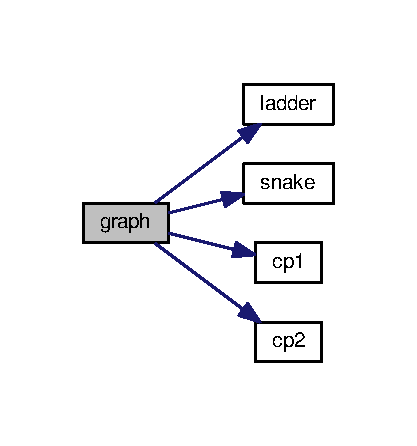
\includegraphics[width=200pt]{SnakeAndLadder_8cpp_ad7d433ae2456eac956adb9e68009763d_cgraph}
\end{center}
\end{figure}


\index{Snake\+And\+Ladder.\+cpp@{Snake\+And\+Ladder.\+cpp}!ladder@{ladder}}
\index{ladder@{ladder}!Snake\+And\+Ladder.\+cpp@{Snake\+And\+Ladder.\+cpp}}
\subsubsection[{\texorpdfstring{ladder(int, int, int, int)}{ladder(int, int, int, int)}}]{\setlength{\rightskip}{0pt plus 5cm}void ladder (
\begin{DoxyParamCaption}
\item[{int}]{s1, }
\item[{int}]{s2, }
\item[{int}]{s3, }
\item[{int}]{s4}
\end{DoxyParamCaption}
)}\hypertarget{SnakeAndLadder_8cpp_a789894102928375db0a1992ef0faddf5}{}\label{SnakeAndLadder_8cpp_a789894102928375db0a1992ef0faddf5}

\begin{DoxyCode}
1453 \{
1454    setcolor(WHITE);
1455    setlinestyle(1,10,3);
1456    line(s1,s2,s3,s4);
1457    line(s1,s2,s1,s2+10);
1458    line(s1,s2,s1+17,s2);
1459    \textcolor{comment}{//circle(s1,s2,3);}
1460 
1461 \}
\end{DoxyCode}
\index{Snake\+And\+Ladder.\+cpp@{Snake\+And\+Ladder.\+cpp}!main@{main}}
\index{main@{main}!Snake\+And\+Ladder.\+cpp@{Snake\+And\+Ladder.\+cpp}}
\subsubsection[{\texorpdfstring{main()}{main()}}]{\setlength{\rightskip}{0pt plus 5cm}void main (
\begin{DoxyParamCaption}
{}
\end{DoxyParamCaption}
)}\hypertarget{SnakeAndLadder_8cpp_acdef7a1fd863a6d3770c1268cb06add3}{}\label{SnakeAndLadder_8cpp_acdef7a1fd863a6d3770c1268cb06add3}

\begin{DoxyCode}
105 \{
106    \hyperlink{SnakeAndLadder_8cpp_a5602f1fbcedd7e2987edb6567dbc8a85}{sohaib}();
107 \}
\end{DoxyCode}


Here is the call graph for this function\+:
\nopagebreak
\begin{figure}[H]
\begin{center}
\leavevmode
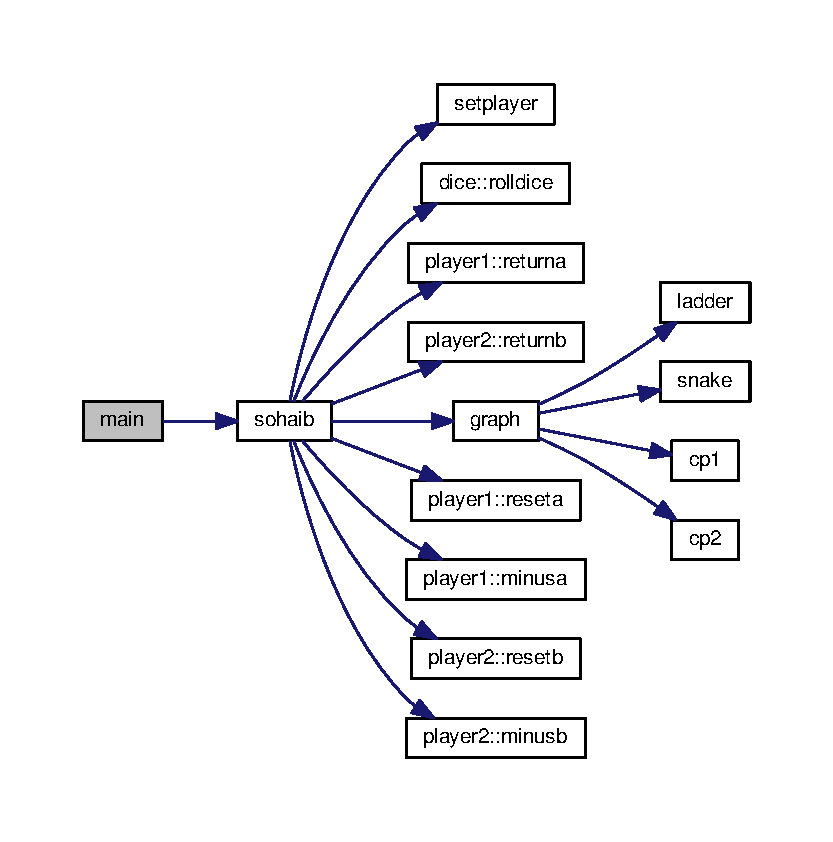
\includegraphics[width=350pt]{SnakeAndLadder_8cpp_acdef7a1fd863a6d3770c1268cb06add3_cgraph}
\end{center}
\end{figure}


\index{Snake\+And\+Ladder.\+cpp@{Snake\+And\+Ladder.\+cpp}!setplayer@{setplayer}}
\index{setplayer@{setplayer}!Snake\+And\+Ladder.\+cpp@{Snake\+And\+Ladder.\+cpp}}
\subsubsection[{\texorpdfstring{setplayer(whoplays)}{setplayer(whoplays)}}]{\setlength{\rightskip}{0pt plus 5cm}{\bf whoplays} setplayer (
\begin{DoxyParamCaption}
\item[{{\bf whoplays}}]{p}
\end{DoxyParamCaption}
)}\hypertarget{SnakeAndLadder_8cpp_aba5a4315ee4edd33d8bf51cf2c5de467}{}\label{SnakeAndLadder_8cpp_aba5a4315ee4edd33d8bf51cf2c5de467}

\begin{DoxyCode}
251 \{
252    \hyperlink{SnakeAndLadder_8cpp_a38df57e4d2dd42645d8726b112528b77}{whoplays} player=p;
253    \textcolor{keywordflow}{return} player;
254 \}
\end{DoxyCode}
\index{Snake\+And\+Ladder.\+cpp@{Snake\+And\+Ladder.\+cpp}!snake@{snake}}
\index{snake@{snake}!Snake\+And\+Ladder.\+cpp@{Snake\+And\+Ladder.\+cpp}}
\subsubsection[{\texorpdfstring{snake(int, int, int, int)}{snake(int, int, int, int)}}]{\setlength{\rightskip}{0pt plus 5cm}void snake (
\begin{DoxyParamCaption}
\item[{int}]{s1, }
\item[{int}]{s2, }
\item[{int}]{s3, }
\item[{int}]{s4}
\end{DoxyParamCaption}
)}\hypertarget{SnakeAndLadder_8cpp_a49b806520ae2a5e43a36b121cb3a0e9c}{}\label{SnakeAndLadder_8cpp_a49b806520ae2a5e43a36b121cb3a0e9c}

\begin{DoxyCode}
1478 \{
1479    setcolor(YELLOW);
1480    setlinestyle(1,10,3);
1481    line(s1,s2,s3,s4);
1482    circle(s1,s2,4);
1483 \}\end{DoxyCode}
\index{Snake\+And\+Ladder.\+cpp@{Snake\+And\+Ladder.\+cpp}!sohaib@{sohaib}}
\index{sohaib@{sohaib}!Snake\+And\+Ladder.\+cpp@{Snake\+And\+Ladder.\+cpp}}
\subsubsection[{\texorpdfstring{sohaib(void)}{sohaib(void)}}]{\setlength{\rightskip}{0pt plus 5cm}void sohaib (
\begin{DoxyParamCaption}
\item[{void}]{}
\end{DoxyParamCaption}
)}\hypertarget{SnakeAndLadder_8cpp_a5602f1fbcedd7e2987edb6567dbc8a85}{}\label{SnakeAndLadder_8cpp_a5602f1fbcedd7e2987edb6567dbc8a85}

\begin{DoxyCode}
110 \{
111    \textcolor{keywordtype}{int} l=VGA,k=VGAMED;
112    initgraph(&l,&k,\textcolor{stringliteral}{"e:\(\backslash\)tc\(\backslash\)bgi"});
113    \textcolor{keyword}{static} \textcolor{keywordtype}{int} x=0;
114    \hyperlink{classdice}{dice} dice1;
115    \hyperlink{classplayer1}{player1} obj1;
116    \hyperlink{classplayer2}{player2} obj2;
117    \textcolor{keywordtype}{int} one=0,two=0,y=0;
118    y=\hyperlink{SnakeAndLadder_8cpp_aba5a4315ee4edd33d8bf51cf2c5de467}{setplayer}(1);
119    g:\textcolor{keywordflow}{if}(x==6)
120    \{
121       \textcolor{keywordflow}{if}(y==0)
122       \{
123     y=\hyperlink{SnakeAndLadder_8cpp_aba5a4315ee4edd33d8bf51cf2c5de467}{setplayer}(0);
124       \}
125       \textcolor{keywordflow}{else}
126       \textcolor{keywordflow}{if}(y==1)
127       \{
128    y=\hyperlink{SnakeAndLadder_8cpp_aba5a4315ee4edd33d8bf51cf2c5de467}{setplayer}(1);
129       \}
130    \}
131    \textcolor{keywordflow}{else}
132    \{
133       \textcolor{keywordflow}{if}(y==0)
134       \{
135     y=\hyperlink{SnakeAndLadder_8cpp_aba5a4315ee4edd33d8bf51cf2c5de467}{setplayer}(1);
136       \}
137       \textcolor{keywordflow}{else}
138       \textcolor{keywordflow}{if}(y==1)
139       \{
140     y=\hyperlink{SnakeAndLadder_8cpp_aba5a4315ee4edd33d8bf51cf2c5de467}{setplayer}(0);
141       \}
142    \}
143 
144    x=int(dice1.\hyperlink{classdice_a967f61248ffb11035c4b2f30b5c32bbb}{rolldice}());
145    one=int(obj1.\hyperlink{classplayer1_a3ab242a781a3cdf6464805b7d343c743}{returna}());
146    two=int(obj2.\hyperlink{classplayer2_a32e37b8a129a947c0c037e0135c51c12}{returnb}());
147    \hyperlink{SnakeAndLadder_8cpp_ad7d433ae2456eac956adb9e68009763d}{graph}(y,one,two);
148    \textcolor{keywordflow}{if}(x==6&&y==0)
149    \{
150       \hyperlink{SnakeAndLadder_8cpp_a949b553aaeb0f5233c17ed4feda5118c}{counter11}=1;
151    \}
152    \textcolor{keywordflow}{if}(x==6&&y==1)
153    \{
154       \hyperlink{SnakeAndLadder_8cpp_ab418db3d9c4875cda2de12f62792cdf1}{counter22}=1;
155    \}
156    \textcolor{keywordflow}{if}(y==0&&\hyperlink{SnakeAndLadder_8cpp_a949b553aaeb0f5233c17ed4feda5118c}{counter11}==1)
157    \{
158       \hyperlink{SnakeAndLadder_8cpp_a22d4ec3074b5dbbbc8a2225b7b23eead}{counter1}=1;
159    \}
160    \textcolor{keywordflow}{if}(y==1&&\hyperlink{SnakeAndLadder_8cpp_ab418db3d9c4875cda2de12f62792cdf1}{counter22}==1)
161    \{
162       \hyperlink{SnakeAndLadder_8cpp_a4a83c833d1791f6e48fd7b0537ca23ec}{counter2}=1;
163    \}
164    \textcolor{keywordflow}{if}(y==0&&\hyperlink{SnakeAndLadder_8cpp_a22d4ec3074b5dbbbc8a2225b7b23eead}{counter1}>=1)
165    \{
166       obj1.\hyperlink{classplayer1_adf9c92711824650060eab93ead7cdd36}{reseta}(x);
167       \textcolor{keywordflow}{if}(one==10)
168       \{
169     obj1.\hyperlink{classplayer1_adf9c92711824650060eab93ead7cdd36}{reseta}(27);
170     cout<<endl<<\textcolor{stringliteral}{"player1 you have moved to 37"};
171       \}
172       \textcolor{keywordflow}{if}(one==55)
173       \{
174     obj1.\hyperlink{classplayer1_adf9c92711824650060eab93ead7cdd36}{reseta}(15);
175     cout<<endl<<\textcolor{stringliteral}{"player1 you have moved to 64"};
176       \}
177       \textcolor{keywordflow}{if}(one==79)
178       \{
179     obj1.\hyperlink{classplayer1_adf9c92711824650060eab93ead7cdd36}{reseta}(10);
180     cout<<endl<<\textcolor{stringliteral}{"player1 you have moved to 89"};
181       \}
182       \textcolor{keywordflow}{if}(one==99)
183       \{
184     obj1.\hyperlink{classplayer1_ab39235bad6825ca38e4373924e492c85}{minusa}(60);
185     cout<<endl<<\textcolor{stringliteral}{"alas! moved to 39"};
186       \}
187       \textcolor{keywordflow}{if}(one==56)
188       \{
189     obj1.\hyperlink{classplayer1_ab39235bad6825ca38e4373924e492c85}{minusa}(30);
190     cout<<endl<<\textcolor{stringliteral}{"alas! moved to 26"};
191       \}
192       \textcolor{keywordflow}{if}(one==77)
193       \{
194     obj1.\hyperlink{classplayer1_ab39235bad6825ca38e4373924e492c85}{minusa}(25);
195     cout<<endl<<\textcolor{stringliteral}{"alas! moved to 52"};
196       \}
197    \}
198    \textcolor{keywordflow}{if}(y==1&&\hyperlink{SnakeAndLadder_8cpp_a4a83c833d1791f6e48fd7b0537ca23ec}{counter2}>=1)
199    \{
200       obj2.\hyperlink{classplayer2_a36cad9ccc12f3df2a45e2cf07f2ff1c7}{resetb}(x);
201       \textcolor{keywordflow}{if}(two==24)
202       \{
203     obj2.\hyperlink{classplayer2_a36cad9ccc12f3df2a45e2cf07f2ff1c7}{resetb}(27);
204     cout<<endl<<\textcolor{stringliteral}{"player2 you have moved to 51"};
205       \}
206       \textcolor{keywordflow}{if}(two==43)
207       \{
208     obj2.\hyperlink{classplayer2_a36cad9ccc12f3df2a45e2cf07f2ff1c7}{resetb}(15);
209     cout<<endl<<\textcolor{stringliteral}{"player2 you have moved to 58"};
210       \}
211       \textcolor{keywordflow}{if}(two==88)
212       \{
213     obj2.\hyperlink{classplayer2_a36cad9ccc12f3df2a45e2cf07f2ff1c7}{resetb}(10);
214     cout<<endl<<\textcolor{stringliteral}{"player2 you have moved to 98"};
215       \}
216       \textcolor{keywordflow}{if}(two==28)
217       \{
218     obj2.\hyperlink{classplayer2_a5d00283bc4c21a964bbd4149192b1537}{minusb}(15);
219     cout<<endl<<\textcolor{stringliteral}{"alas! moved to 13"};
220       \}
221       \textcolor{keywordflow}{if}(two==69)
222       \{
223     obj2.\hyperlink{classplayer2_a5d00283bc4c21a964bbd4149192b1537}{minusb}(30);
224     cout<<endl<<\textcolor{stringliteral}{"alas! moved to 39"};
225       \}
226       \textcolor{keywordflow}{if}(two==99)
227       \{
228     obj2.\hyperlink{classplayer2_a5d00283bc4c21a964bbd4149192b1537}{minusb}(60);
229     cout<<endl<<\textcolor{stringliteral}{"alas! moved to 39"};
230       \}
231    \}
232    \textcolor{keywordflow}{if}(one>=100)
233    \{
234       cout<<\textcolor{stringliteral}{"}
235 \textcolor{stringliteral}{congratulations player 1 have won"};
236       \textcolor{keywordflow}{goto} b;
237    \}
238    \textcolor{keywordflow}{if}(two>=100)
239    \{
240       cout<<\textcolor{stringliteral}{"}
241 \textcolor{stringliteral}{congratulations player 2 have won"};
242       \textcolor{keywordflow}{goto} b;
243    \}
244    \textcolor{keywordflow}{if}((one<101&&two<101)&&(one>=0&&two>=0))
245    \{
246       \textcolor{keywordflow}{goto} g;
247    \}
248    b:getch();
249 \}
\end{DoxyCode}


Here is the call graph for this function\+:
\nopagebreak
\begin{figure}[H]
\begin{center}
\leavevmode
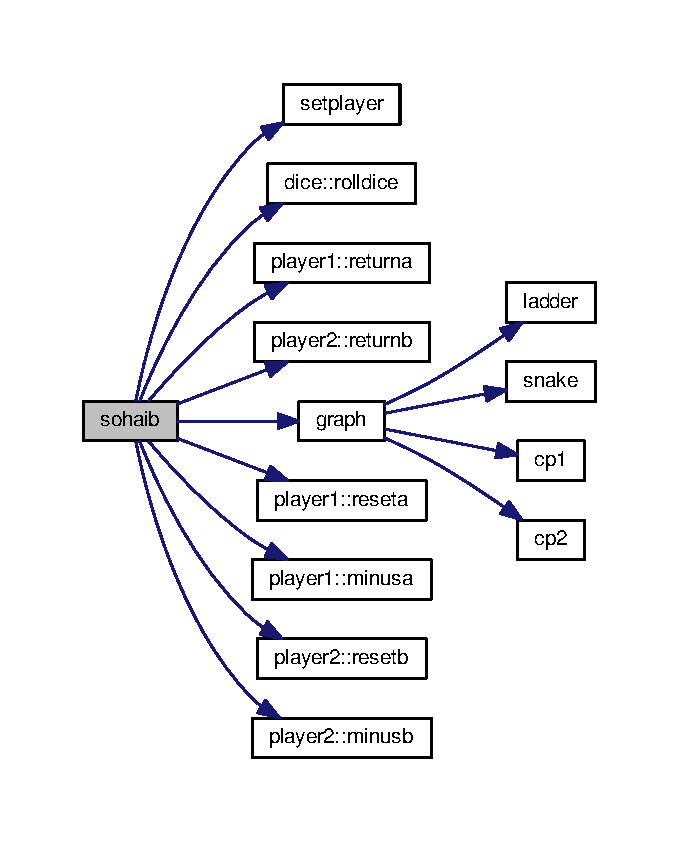
\includegraphics[width=326pt]{SnakeAndLadder_8cpp_a5602f1fbcedd7e2987edb6567dbc8a85_cgraph}
\end{center}
\end{figure}




\subsection{Variable Documentation}
\index{Snake\+And\+Ladder.\+cpp@{Snake\+And\+Ladder.\+cpp}!counter1@{counter1}}
\index{counter1@{counter1}!Snake\+And\+Ladder.\+cpp@{Snake\+And\+Ladder.\+cpp}}
\subsubsection[{\texorpdfstring{counter1}{counter1}}]{\setlength{\rightskip}{0pt plus 5cm}int counter1 =0}\hypertarget{SnakeAndLadder_8cpp_a22d4ec3074b5dbbbc8a2225b7b23eead}{}\label{SnakeAndLadder_8cpp_a22d4ec3074b5dbbbc8a2225b7b23eead}
\index{Snake\+And\+Ladder.\+cpp@{Snake\+And\+Ladder.\+cpp}!counter11@{counter11}}
\index{counter11@{counter11}!Snake\+And\+Ladder.\+cpp@{Snake\+And\+Ladder.\+cpp}}
\subsubsection[{\texorpdfstring{counter11}{counter11}}]{\setlength{\rightskip}{0pt plus 5cm}int counter11 =0}\hypertarget{SnakeAndLadder_8cpp_a949b553aaeb0f5233c17ed4feda5118c}{}\label{SnakeAndLadder_8cpp_a949b553aaeb0f5233c17ed4feda5118c}
\index{Snake\+And\+Ladder.\+cpp@{Snake\+And\+Ladder.\+cpp}!counter2@{counter2}}
\index{counter2@{counter2}!Snake\+And\+Ladder.\+cpp@{Snake\+And\+Ladder.\+cpp}}
\subsubsection[{\texorpdfstring{counter2}{counter2}}]{\setlength{\rightskip}{0pt plus 5cm}int counter2 =0}\hypertarget{SnakeAndLadder_8cpp_a4a83c833d1791f6e48fd7b0537ca23ec}{}\label{SnakeAndLadder_8cpp_a4a83c833d1791f6e48fd7b0537ca23ec}
\index{Snake\+And\+Ladder.\+cpp@{Snake\+And\+Ladder.\+cpp}!counter22@{counter22}}
\index{counter22@{counter22}!Snake\+And\+Ladder.\+cpp@{Snake\+And\+Ladder.\+cpp}}
\subsubsection[{\texorpdfstring{counter22}{counter22}}]{\setlength{\rightskip}{0pt plus 5cm}int counter22 =0}\hypertarget{SnakeAndLadder_8cpp_ab418db3d9c4875cda2de12f62792cdf1}{}\label{SnakeAndLadder_8cpp_ab418db3d9c4875cda2de12f62792cdf1}

%--- End generated contents ---

% Index
\backmatter
\newpage
\phantomsection
\clearemptydoublepage
\addcontentsline{toc}{chapter}{Index}
\printindex

\end{document}
